% Compilation: <leader>ll
\documentclass[12pt,a4paper,openany,english]{extbook}
\usepackage[a4paper,includeheadfoot,margin=2.50cm]{geometry}


% By default, LaTeX tries to stretch whitespace between paragraphs on a page in order to reduce whitespace at the end of the page. This sometimes gives ugly results. The following command disables that stretching.
\raggedbottom % Don't reduce whitespace at the end of a page.

\renewcommand{\baselinestretch}{1.2}  % stretch horizontal space between everything by 20%


\usepackage[hyphens]{url} % Break line on hyphens in long urls
\usepackage{graphicx}
\graphicspath{{images/}}
\usepackage{pdfpages}
\usepackage{enumitem}
\usepackage{float}
\usepackage{caption}
\usepackage{subcaption}
\usepackage[toc,page]{appendix}
\usepackage{fontspec}
\usepackage[T1]{fontenc}

% Don't indent table of contents, list of figures, and list of tables
\usepackage{tocloft}
\setlength{\cftsecindent}{0pt}    % Remove indent for \section in Table of Contents
\setlength{\cftsubsecindent}{0pt} % Remove indent for \subsection in Table of Contents
\setlength{\cftfigindent}{0pt}    % remove indentation from figures in List of Figures
\setlength{\cfttabindent}{0pt}    % remove indentation from tables in List of Tables

\usepackage{parskip} % Add space between two paragraphs and don't indent the first line of the paragraph

% To generate fake lorem ipsum text
% \usepackage{lipsum}

%
% UGent style guide
%
\setmainfont[
	Path=fonts/,
	BoldFont      =UGentPannoText-SemiBold.ttf,
	ItalicFont    =UGentPannoText-Normal.ttf,
	ItalicFeatures={FakeSlant=0.3},
	BoldItalicFont=UGentPannoText-SemiBold.ttf,
    BoldItalicFeatures={FakeSlant=0.3},
]{UGentPannoText-Normal.ttf}
\urlstyle{same} % Also use the default font for URLs


% If you want left justified text, uncomment the line below.
%\usepackage[document]{ragged2e} % Left justify all text

% Style Chapter titles so they have the chapter number in grey.
\usepackage{color}
\definecolor{chaptergrey}{rgb}{0.5,0.5,0.5}
\usepackage[explicit, pagestyles]{titlesec}
\titleformat{\chapter}[display]{\bfseries}{\color{chaptergrey}\fontfamily{pbk}\fontsize{80pt}{100pt}\selectfont\thechapter}{0pt}{\Huge #1}
\titlespacing*{\chapter}{0pt}{-80pt}{30pt}


% Header showing chapter number and title and footer showing page number
\newpagestyle{fancy}{%
  \sethead{} % left
          {} % center
          {\Large\thechapter~~\chaptertitle} %right
  \setfoot{} % left
          {\thepage} % center
          {} %right
  \setheadrule{0pt}
}
\pagestyle{fancy}

% Header showing chapter title and footer showing page number
\newpagestyle{numberless}{%
  \sethead{} % left
          {} % center
          {\Large\chaptertitle} %right
  \setfoot{} % left
          {\thepage} % center
          {} %right
  \setheadrule{0pt}
}

% We use the package `minted` for modern code highlighting.
\usepackage[newfloat,chapter]{minted}
% \SetupFloatingEnvironment{listing}{name=Codefragment, listname=Lijst van codefragmenten}
\SetupFloatingEnvironment{listing}{name=Codefragment, listname=List of Code Fragments} % lang:english


\PassOptionsToPackage{hyphens}{url}
\usepackage{hyperref}
\usepackage{url}

\usepackage[numbers]{natbib}       % For bibliography; use numeric citations
\bibliographystyle{IEEEtran}
\usepackage[nottoc]{tocbibind}     % Put Bibliography in ToC

%
% Defines \checkmark to draw a checkmark
%
\usepackage{tikz}
\def\checkmark{\tikz\fill[scale=0.4](0,.35) -- (.25,0) -- (1,.7) -- (.25,.15) -- cycle;}

%
% For tables
%
\usepackage{booktabs}
\usepackage{array}
\usepackage{ragged2e}  % for '\RaggedRight' macro (allows hyphenation)
\newcolumntype{L}[1]{>{\raggedright\let\newline\\\arraybackslash\hspace{0pt}}m{#1}}
\newcolumntype{C}[1]{>{\centering\let\newline\\\arraybackslash\hspace{0pt}}m{#1}}
\newcolumntype{R}[1]{>{\raggedleft\let\newline\\\arraybackslash\hspace{0pt}}m{#1}}

%
% Support for splitting Dutch words correctly
%
\usepackage{polyglossia}
% \setdefaultlanguage[babelshorthands=true]{dutch} % lang:dutch
\setmainlanguage{english}                       % lang:english

% Manually specify additional hypnations for words
%
% Translated strings. If these aren't set, the English words are used.
%
% \addto\captionsenglish{\renewcommand{\contentsname}{Inhoudsopgave}}   % lang:dutch

% Fix error "Package hyperref Warning: The anchor of a bookmark and its parent's must not be the same. Added a new anchor on ..."
\newcommand{\sectionbreak}{\phantomsection}

% \renewcommand\appendixtocname{Bijlagen}                     % lang:dutch
% \renewcommand\appendixpagename{Bijlagen}                    % lang:dutch


\usepackage[toc,acronym]{glossaries}  % for list of acronyms
\makeglossaries                       % start internal list of acronyms


%
% Set the title and your name
%
%%%%%%%%%%%%%%%%%%%%%%%%%%%%%%%%%%%%%%%%%%%%%%%%%%%%%%%%%%%%%%%%%%%%%%
%
% Add the specific info for your thesis
%
%%%%%%%%%%%%%%%%%%%%%%%%%%%%%%%%%%%%%%%%%%%%%%%%%%%%%%%%%%%%%%%%%%%%%%

\title{Advancing the I2C proposal for WebAssembly System Interface}
\author{Friedrich Vandenberghe}

%%%%%%%%%%%%%%%%%%%%%%%%%%%%%%%%%%%%%%%%%%%%%%%%%%%%%
% Add all the acronyms you use in your thesis here. %
% These will be added to the List of Acronyms       %
%%%%%%%%%%%%%%%%%%%%%%%%%%%%%%%%%%%%%%%%%%%%%%%%%%%%%

%          label acronym
\newacronym{ABI}{ABI}{application binary interface}
\newacronym{I2C}{I2C}{Inter-Integrated Circuit}
\newacronym{OS}{OS}{Operating System}
\newacronym{SWD}{SWD}{Serial Wire Debug}
\newacronym{SVD}{SVD}{System View Description}
\newacronym{GPIO}{GPIO}{general-purpose input/output}
\newacronym{UART}{UART}{universal asynchronous receiver-transmitter}
\newacronym{SPI}{SPI}{Serial Peripheral Interface}
\newacronym{Wasm}{Wasm}{WebAssembly}
\newacronym{IDL}{IDL}{Interface Description Language}
\newacronym{WASI}{WASI}{WebAssembly System Interface}
\newacronym{WIT}{WIT}{Wasm Interface Type}
\newacronym{MCU}{MCU}{Microcontroller Unit}
\newacronym{SIG}{SIG}{Special Interest Group}
\newacronym{VM}{VM}{Virtual Machine}
\newacronym{HAT}{HAT}{Hardware Attached on Top}
\newacronym{HAL}{HAL}{Hardware Abstraction Layer}
\newacronym{API}{API}{Application Programming Interface}
\newacronym{SDA}{SDA}{Serial Data Line}
\newacronym{SCL}{SCL}{Serial Clock Line}
\newacronym{ACK}{ACK}{Acknowledgement}
\newacronym{NACK}{NACK}{Negative-acknowledgement}
\newacronym{SMBus}{SMBus}{System Management Bus}
\newacronym{WAMR}{WAMR}{WebAssembly Micro Runtime}


%
%  END OF HEADER
%  The actual latex document content starts here.
%
\begin{document}

\frontmatter
\pagestyle{empty}

% Download the cover sheet from Plato
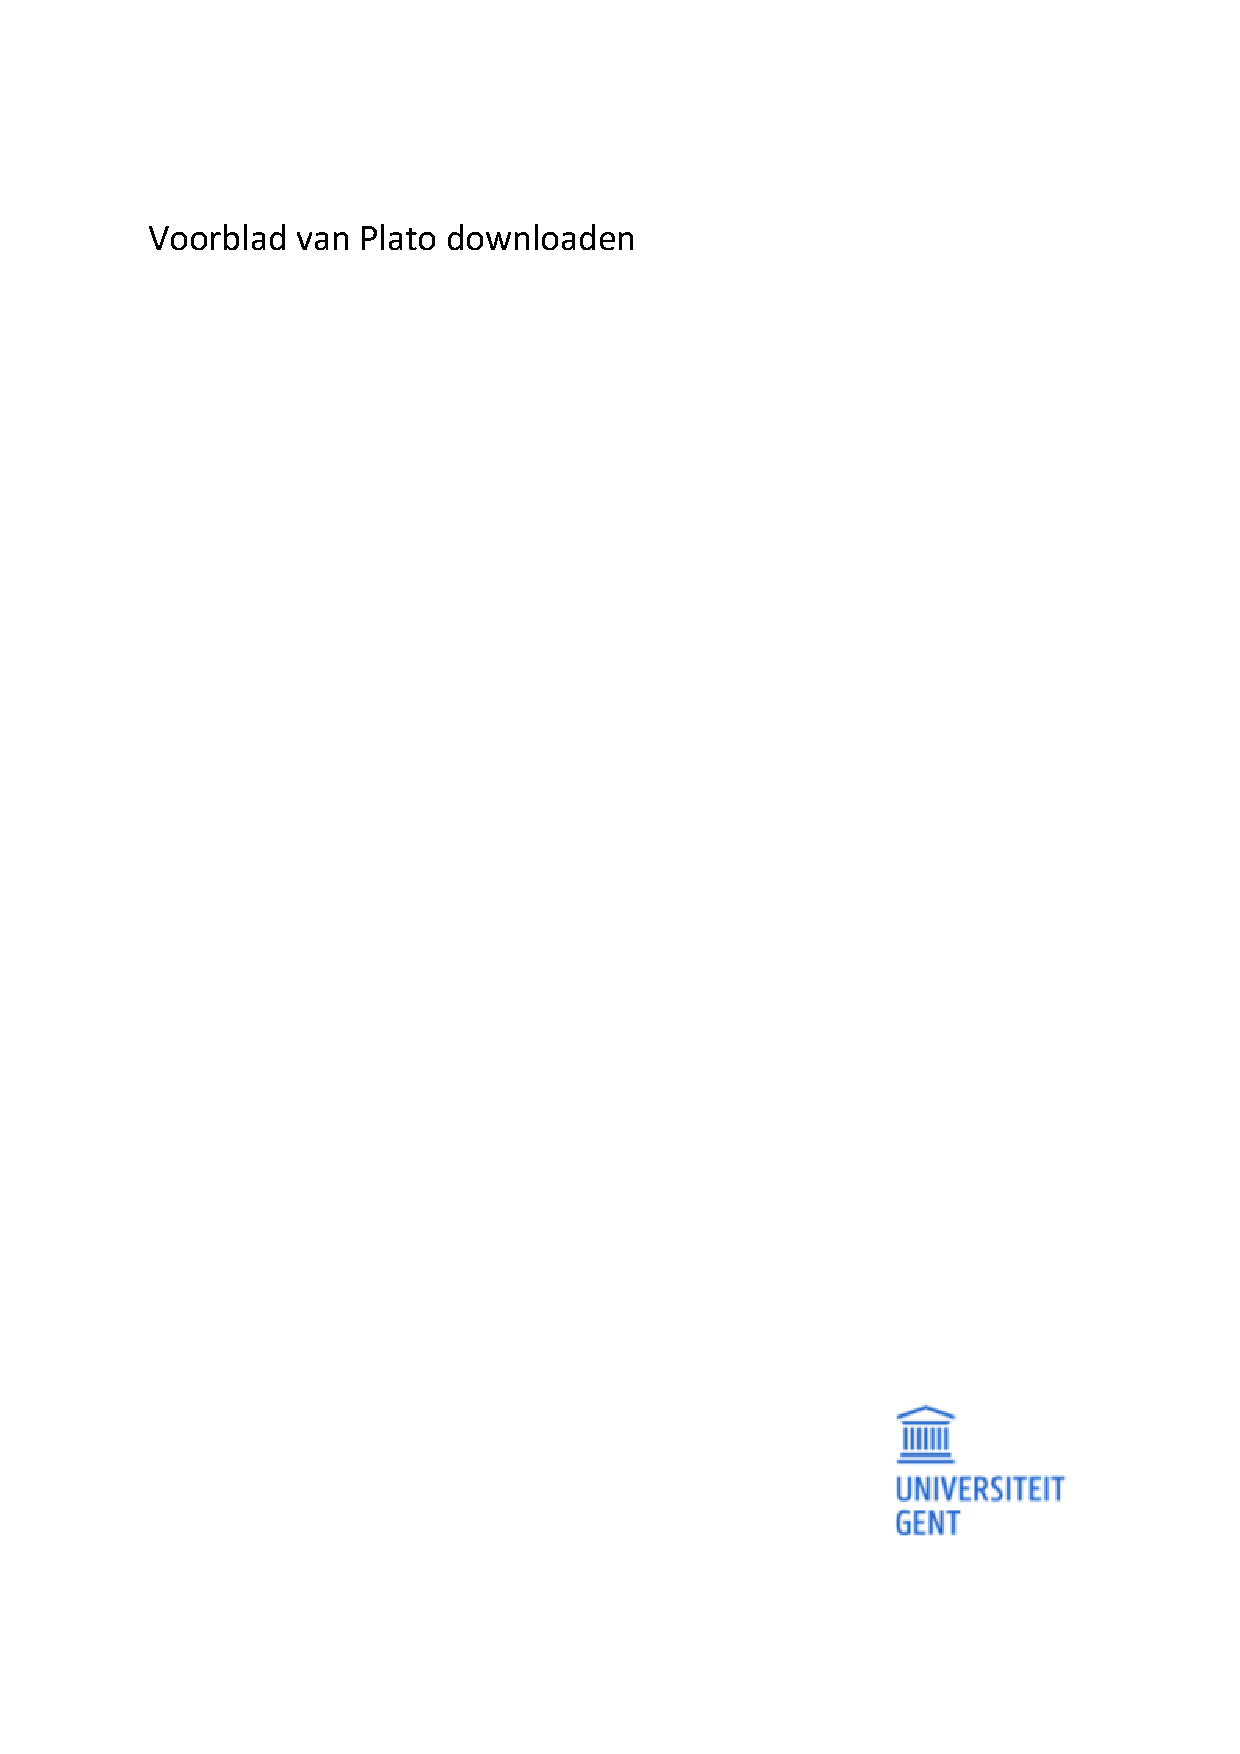
\includepdf{cover-sheet.pdf}

\chapter*{Dankwoord}

Allereerst wil ik mijn promotoren, prof. dr. Bruno Volckaert en prof. dr. ir. Filip De Turck, en begeleiders, dr. ing. Merlijn Sebrechts en dr. ing. Tom Goethals, bedanken. Zonder hen zou deze masterproef nooit tot stand gekomen kunnen zijn. In het bijzonder wil ik dr. ing. Merlijn Sebrechts bedanken voor de opvolging en het oneindige geduld om mijn zinnen met een passive voice aan te duiden. 

Daarnaast wil ik graag mijn ouders bedanken voor de steun, en het proeflezen. Zonder hen zou dit ook nooit tot stand gekomen kunnen zijn en waren er ongetwijfeld nog talloze grammaticale fouten aanwezig. 

Tot slot wil ik ook graag iedereen in de Bytecode Alliance waarmee ik in contact gekomen ben bedanken voor diens onschatbare feedback en hulp, hieruit wil ik Dan Gohman, Chris Woods en Maximilian Seidler uitlichten.

\chapter*{Permission for Usage}

The author gives permission to make this master’s thesis available for consultation and to copy parts of this master’s thesis for personal use. Every other use is subject to copyright terms, in particular with regard to the obligation to explicitly state the source when quoting results from this master’s thesis.


\chapter*{Abstract - Dutch}
\chaptermark{Abstract - Dutch}
\addcontentsline{toc}{chapter}{Abstract - Dutch}


\chapter*{Abstract - English}
\chaptermark{Abstract - English}
\addcontentsline{toc}{chapter}{Abstract - English}



% How to add the extended abstract:
%
% You should write the extended abstract as a separate overleaf project. Then compile it there, download the PDF, and upload it to this project.
%
% Use the "IEEE conference proceedings template" to create the extended abstract project. 
% https://www.overleaf.com/latex/templates/ieee-conference-template/grfzhhncsfqn
%
% Then download the final PDF, upload it to the root of this project, and point the statement below to the correct file.


% How to add the extended abstract:
%
% You should write the extended abstract as a separate overleaf project. Then compile it there, download the PDF, and upload it to this project.
%
% Use the "IEEE conference proceedings template" to create the extended abstract project. 
% https://www.overleaf.com/latex/templates/ieee-conference-template/grfzhhncsfqn
%
% Then download the final PDF, upload it to the root of this project, and point the statement below to the correct file.

\tableofcontents\newpage
\listoffigures\newpage
\listoftables\newpage
%%%%%%%%%%%%%%%%%%%%%%%%%%%%%%%%%%%%%%%%%%%%%%%%%%%%%%%%%%%%%%%
%                                                             %
% Note: To add or remove acronyms, modify `personal_data.tex` %
%                                                             %
%%%%%%%%%%%%%%%%%%%%%%%%%%%%%%%%%%%%%%%%%%%%%%%%%%%%%%%%%%%%%%%

% Print the glossary
% \printglossary[type=\acronymtype, title={Lijst van afkortingen}]
\printglossary[type=\acronymtype, title={List of Acronyms}] % English

\glsaddallunused[\acronymtype]                              % make sure all unused acronyms are in list

\setlist[description]{style=standard} % reset list settings back to default

% list all code listings
\listoflistings\newpage
\newpage

%
% Include the main chapters of the thesis below
% Note: it's best to avoid spaces in filenames as Latex might complain about them.
%
\mainmatter
\pagestyle{fancy} % Use header
% Moet zeker goed verwoord zijn
\chapter{Introduction}
\label{chap:intro}

[secties zijn tijdelijk, en puur om aan te tonen dat tekst voor "onderzoeksvragen" nog niet klaar genoeg is]
\section{WIP}
% Dit kan gezien worden als een omgekeerde driehoek

% 1. Wat is het maatschappelijke probleem?
% 	1. Voorbeeld: Updaten van auto's
% 	2. Er mag gelinkt worden met nieuwsartikels

There are countless software solutions running on critical hardware, where sudden failure could result in the loss of people's live, e.g. programs guiding surgeons during operations or cars. Furthermore, in the case of cars, there's a clear trend towards more advanced infotainment systems and to update these remotely without the need to visit an auto mechanic. When such an update fails to perform, it should be possible to rollback unbeknownst to the driver.

% TODO: Brug naar lange termijn onderhoud
% 2. Firmware, heel lang onderhouden en zo brugje naar Wasm maken
% 	1. Probleem: Wasm heeft geen manier om met hardware te praten
% 	2. En dan dit probleem uitdiepen: Wasi, I2C

In addition, with the advent of generational AI's like ChatGPT, worldwide GPU usage has exploded. Directly translating in an explosion of energy and water usage to run all and cool all this harware inside data-centres. Sadly, these GPUs have long-lasting periods of idly running, waiting for requests. It should be possible to start a GPU when running a request, but otherwise keep it off, without significant overhead in terms of latency.

% TODO: Hierop is de hele korte startup times en overhead van Wasm ook de oplossing

\section{Onderzoeksvragen}
% TODO: 3. Onderzoeksvragen en kort overzicht
% 	1. Hoe kan het secure gebeuren?
% 	2. Wat is de performance?


% \setcounter{page}{1}
\chapter{Background}
\label{chap:bg}

\section{WebAssembly}
\label{chap:wasm}
% [Algemene uitleg van wat WebAssembly is en waarom we het buiten het web willen kunnen gebruiken. Hiervoor wordt er dan verwezen naar de lagere memory footprint ten opzichte van docker. Alsook moet er verteld worden wat de previews zijn en de timeline van wanneer ze gereleased zijn. Spinup time is ook een zeer belangrijke om te vermelden.]

\gls{Wasm} is a binary instruction format for a stack-based \gls{VM}. It is designed as a portable compilation target for programming languages. Binaries have a \texttt{.wasm} file extension, there's also a textual representation which has a \texttt{.wat} extension. This enables deployment on the web for client and server applications. Examples of web applications using this technology are Adobe Photoshop~\cite{wasm:ps} and Google Earth~\cite{wasm:ge}.

Although the name implies it, \gls{Wasm} is not merely limited to the web. There are runtimes that enable execution on a myriad of platforms, ranging from Linux devices to smartphones or even microcontrollers. Via a system interface that enables direct \gls{OS} communication, called \gls{WASI}.

\subsection{JavaScript integration}

Initially, \gls{Wasm} was designed for near-native code execution speed in the web browser\footnote{To be precise, it's the JavaScript engine inside the browser that added support for WebAssembly.}. Therefore, it was designed to run alongside JavaScript, allowing both to work together. In this early stage, compiling to \gls{Wasm} was supplemented with the generation of the required JavaScript glue code. For this, the emscripten~\cite{gh:emscripten} compiler is used.

Outside the web browser, there are also platforms that provide a JavaScript runtime environment, i.e. Node.js~\cite{nodejs} and Deno~\cite{deno}. They both, too, have \gls{Wasm} support, but no manner of accessing \gls{OS} functionality directly on its own. For this the \gls{WASI} \gls{API} needs to be utilized.

For \texttt{Node.js}, integration with \gls{WASI} is experimental and does not provide the comprehensive security properties provided by dedicated \gls{WASI} runtimes. It is uncertain whether full support will ever be implemented. In \texttt{Deno} official support has been deprecated due to a lack of interest~\cite{deno:wasi}.

\clearpage
\section{WebAssembly System Interface}
\label{sec:wasi}

\gls{WASI}~\cite{wasi} is a modular collection of \gls{API} proposals defined with the \gls{WIT} IDL. It provides a secure and portable way to access several operating-system-like features such as filesystems, networking, clocks and random numbers. This collection is developed under the governance of the \gls{WASI} Subgroup, a subgroup of the W3C's, the World Wide Web Consortium, WebAssembly Community Group.

This subgroup doesn't provide any implementations, for this the Bytecode Alliance~\cite{ba:announce} exists, a nonprofit organization of companies containing Fastly, Fermyon, Cosmonic, Intel, Microsoft, Siemens and more. Inside this organization, there's also a subcommunity of people interested in the combination of \gls{Wasm} and embedded devices. To ratify this subcommunity, a request for a \gls{SIG} Embedded has been opened with the Bytecode Alliance.

\subsection{Design principles}
\label{sec:design}

The following design principles are core:

\begin{itemize}
    \item Capability-based security: All access to external resources is provided by capabilities.
    \item Interposition: A Webassembly instance can implement a given WASI interface, and the consumer WebAssembly instance can then use this implementation transparently.
    \item Compatibility: If possible, keep the \gls{API} free of Compatibility concerns, and provide compatibility through libraries.
    \item Portability: The exact meaning of this is specific to each \gls{API}, but in globo it means that no engine should need to implement every \gls{API} in \gls{WASI}.
    \item Modularity: The component model's worlds mechanism is used, in order to allow specific sets of APIs to be described which meet the needs of different environments. See chapter~\ref{chap:component_model}.
\end{itemize}

From these, capability-based security can be seen as the key defining feature. Capability-based security dictates that access to external resources must be denied, unless it is authorized via capabilities~\cite{cap-security}. In the context of \gls{WASI}, there are two kinds of capabilities:

\begin{itemize}
    \item Handles: Dynamically indetify and provide access to resources via a 32-bit integer index. This is analogue to file descriptors.
    \item Link-time capabilities: Functions that require no handle arguments. These are used in situations where it's not necessary to identify more than one instance of a resource at runtime. Used sparingly.
\end{itemize}

For this security model to work correctly, its default to block all external accesses must be airtight, i.e. the runtime needs to be secure.

\subsection{The standardization process}

The \gls{WASI} subgroup is further split up into the Community Group and the Working Group. The purpose of the Community Group is to attempt to address all concerns, but no 100\% consensus is needed. The Working Group, on the other hand, is there to finalize and ratify mostly complete specifications plus test suites from the Community Group.

% This means that they are responsible for any proposed changes to this collection of interfaces to be thoroughly vetted by the community.

The process is split up into five stages of standardization:

\begin{description}
    \item[Phase 0.] Pre-Proposal: The Community Group decides whether the pre-proposal is in scope for \gls{WASI}.
    \item[Phase 1.] Proposement of the feature: An overview document must be produced that specifies the feature with reasonably precise and complete language.
    \item[Phase 2.] Specification text is available: A test suite should be added, and it should pass on the prototype or some other implementation.
    \item[Phase 3.] The specification gets implemented by engines.
    \item[Phase 4.] The feature is being standardized: Ownership gets transferred from the Community Group to the Working Group, and two or more Web \gls{VM}'s have implemented the feature.
    \item[Phase 5.] The feature is standardized: Editors perform final editorial tweaks and merge the feature into the main branch of the primary specification repository.

\end{description}

To go from the one stage to the following, a vote in the subgroup needs to be passed. Except to enter phase 0, here the proposal is still merely an idea.

\subsection{WIT}
\label{sec:wit}
% [Schetsen wat WIT is en kort hoe de syntax in elkaar zit. Misschien dat het ook handig kan zijn om uit te leggen hoe dependencies in WIT gemanaged worden.]

\gls{WIT} is an \gls{IDL}. This means that it is a format that defines how the interface of a component should look like. To this end, it uses the following set of concepts: types, functions, interfaces, worlds and packages. From these, worlds are the most key.

A world describes the capabilities and needs of a component - it says which interfaces are available for outside code to call, the \texttt{export}s, and which interfaces it depends on, the \texttt{import}s. Thus, only the surface of a component is defined, not the internal behaviour. The internal behaviour is determined when the world is targeted by a component an application or library developer creates. For a component to run, its imports must be fulfilled, by a host or by other components. \\
On the other hand, a world defines an environment in which a component can be instantiated, and its functionality can be invoked.

Regarding the other concepts, functions can only be declared as part of an interface, or as an import or export in a world. Finally, a package is not a world, but can be seen as more like a namespace. It's a way of grouping related interfaces and worlds together for ease of discovery and reference.

\gls{WIT} also provides built-in types, including primitives like signed and unsigned integer types, floats, strings, and more complex types like results, options and lists. In these, there are two small intricacies worth pointing out. First, both the \texttt{char} and \texttt{string} types are Unicode. Second, there's the user-defined \texttt{resource} type. This type can be seen as an object that implements an interface, and therefore behaviour is only exposed through methods.


To make managing dependencies inside your \gls{WIT} definition easier, the \texttt{wit-deps}~\cite{gh:wit_deps} project can be used. It makes it possible to lock your dependencies to a certain version and to check if they're the most recent one.

\subsubsection{\texttt{witx}}

In older tooling, it is possible to come across \texttt{witx} instead of \gls{WIT}. This was the \gls{IDL} used during \texttt{Preview 1}. It was derived from \texttt{wat}, see chapter~\ref{chap:wasm}, and had a low-level C-like type system that emphasized raw pointers, and callees were expected to have access to the entir lineair memory of the caller.

\subsection{Versions}
\label{sec:versions}
At the time of writing, \gls{WASI} is in \texttt{Preview 2}. The flagship feature of this preview is the release of the component model, see section~\ref{chap:component_model}. Furthermore, two \gls{WIT} worlds are now included:

\begin{itemize}
    \item \texttt{wasi-cli}: A command-line interface, roughly corresponding to \texttt{POSIX}.
    \item \texttt{wasi-http}: An \texttt{HTTP} proxy.
\end{itemize}

The major banner of the upcoming \texttt{0.3} is asynchronous support. The exact details of what this asynchrony entails is yet to be determined. Following up will be a stable 1.0 release.

\newpage

\subsection{Runtimes}
\label{sec:runtimes}
% [Wasmtime uitvoerig bespreken, maar ook de meest belangrijke andere runtimes. Het is niet de bedoeling om echt in depth te gaan vergelijken en te benchmarken, maar om gewoon wat te schetsen wat er allemaal is. Daarnaast ook vertellen in welke mate, en hoe, je een preview2 component op een runtime kan laten draaien dat geen support heeft voor het component model. Misschien ook kort iets rond changes die in Wasmtime kunnen gebeuren om meer embedded devices te supporten.]

A runtime system is a binary that is accountable for the running of \gls{Wasm} binaries. Analogue to the role of a hypervisor for a virtual machine. Depending on the capabilities of the runtime, it contains the following noteworthy high-level items:

\begin{description}
    \item[Engine:] An engine stores and configures global compilation settings like optimization level, enabled wasm features, etc.
    \item[Module:] This represents a compiled form of the input preview 1 wasm module.
    \item[Component:] A compiled preview 2 component ready to be instantiated.
    \item[Linker:] A component-style location for defining host functions. This is not the same as \texttt{wasmtime::Linker} for modules.
    \item[Instance:] An instance of a component, or module, is the actual object on which the functions are called.
    \item[Store:] The store owns the instances, functions, globals, etc.
\end{description}

The Bytecode Alliance maintains two runtimes, Wasmtime~\cite{wasmtime} and WAMR~\cite{gh:wamr}.

Wasmtime can be seen as a general-purpose runtime, focussing on server-side and non-web embeddings with components. It has full component model support, first-class support for eight languages, and community support for a further two. This makes it the de-facto runtime.

On the other hand, \gls{WAMR} is specifically designed to be as lightweight as possible, targeting embedded devices and the edge. This translates itself into the provided features and the supported guest languages. Support for the component model is planned for the end of 2024, and it only has robust support for C/C++. A toolkit for Rust has been published in March 2024~\cite{gh:wrsdk}, but this is still novel.

In Rust, the standard library, abbreviated as \texttt{std}, is a set of minimal shared abstractions for the broader Rust ecosystem. This library is enabled by default, and can be opted out via the \texttt{no\_std} attribute. Rejection is useful when targeting a platform that does not support the library or purposfully doesn't use the capabilities of \texttt{std}. Historically, the community surrounding Wasmtime has been strongly opposed to the inclusion of a \texttt{no\_std} build. This is no longer the case. When such a build will eventually be available, the gap between Wasmtime and \gls{WAMR} will be reduced.

Besides these two, there are numerous ones provided by other parties, in varying degrees of completeness, targeting other use-cases. There's for example Jco~\cite{jco}, specialized for JavaScript, componentize.py~\cite{gh:cpy}, for Python, or Chicory~\cite{yt:chicory}, which runs on the Java \gls{VM}. These are out-of-scope for this dissertation.

\newpage

\subsection{Alternatives}

% 2. Bredere exploratie voor alternatieve oplossingen
% 	1. Hoe I2C aangesproken wordt vanuit nodejs (antwoord: ze geven linux handle) en via linux
% 	2. WebUSB: Dit is via js dus barf
% 	3. Hier kan er hard gegaan worden op linken met academische artikels

Inside the \gls{Wasm} ecosystem, there's mechanoid~\cite{mechanoid}, a framework for applications on embedded systems and \gls{IoT} devices that had its first release in March 2024. The framework itself is written in Go, and it has builtin support for the wazero~\cite{wazero} and wasman~\cite{gh:wasman} runtimes. Both runtimes specifically designed for Go developers. It doesn't use \gls{WASI}, nor does it have any plans for this. This makes it unsuitable for us.

In the Node.js ecosystem, the most prominent package available for an \gls{I2C} connection is \texttt{i2c-bus}~\cite{gh:i2c-bus}. This is an addon written in C++ that operates directly on a given file descriptor.

For the web, \texttt{chirimen-drivers}~\cite{chirimen} could be used, but the documentation is completely written in Japanese. Alternatively, combined use of the WebUSB and Web Serial \gls{API} could be done, but unfortunately the Web Serial \gls{API} is only available in Chrome, Edge and Opera.

On Windows, \gls{I2C} communication can be performed via the \texttt{HIDI2C.sys}~\cite{windows:i2c} driver. Linux allows access to a device from userspace, through the \texttt{/dev}~\cite{linux:i2c} interface. For this, the \texttt{i2c-dev} kernel module needs to be loaded. Each registered adapter gets a number, starting at 0. To start the communication, first the device file needs to be opened and then the target address must be set with \texttt{ioctl(file, I2C\_SLAVE, addr)}. Finally, on macOS the connection is controlled with the \texttt{IOI2CInterface.h}~\cite{macos:i2c} interface inside the \texttt{IOKit} framework.


\clearpage
\section{The Component Model}
\label{chap:component_model}

% [Wat is het component model en waarom willen we het. Ook vertellen dat je het kan zien als een guest/host-architectuur, maar dat het perfect mogelijk is om meerdere componenten samen te weven.]

The WebAssembly Component Model is an architecture for building interoperable \gls{Wasm} liraries, applications and environments. These components can be seen as a wrapper around a core module, or other components, which express their interfaces and dependencies via \gls{WIT} and the canonical \gls{ABI}. Unlike core modules, components may not export \gls{Wasm} memory, reinforcing \gls{Wasm} sandboxing and facilitating interoperation between languages with different memory assumptions.

An \gls{ABI} can be seen as an agreement on how to pass around data in a binary format, specifically concerned with the data layout at the bits-and-bytes level. The Canonical \gls{ABI} defined by the component model, specifies how the \gls{WIT} type definitions are translated to bits and bytes. Internally, a C and a Rust component might represent strings in a quite different way, but the canonical \gls{ABI} provides a format for them to pass strings across the boundary between them.

In regard to \gls{WASI}, the component model is the staple feature of its second preview, but it is possible to make use of the \gls{WASI} interfaces without the component model, and thus this model is entirely optional. By way of comparison to a traditional \gls{OS}, the Component Model fills the role of an \gls{OS}'s process model, defining how processes start up and communicate with each other, while \gls{WASI} fills the role of an \gls{OS}'s many I/O interfaces.

To compose multiple components together \texttt{wasm-tools}~\cite{gh:wt} can be used, or visually using the builder~\cite{builder} app. Specifically for Rust, \texttt{cargo-component}~\cite{gh:cc} is also an option.

\subsection{Toolchain}
\label{sec:guest}
% [Op welke manieren kan je allemaal code schrijven dat dan naar een preview 2 component gecompileerd kan worden. Verschillende tooling over programmeertalen heen de specifieke voor Rust. Alsook hoe we van preview1 component naar preview2 kunnen gaan.]

In Rust, \texttt{cargo-component} can be used to compile code to a preview 2 component. In essence, compiling to \texttt{Preview 2} means compiling to \texttt{wasm32-wasi} and then converting it to a component via an adapater and the \texttt{wasm-tools component new} subcommand. This component then adheres to the \gls{WIT} interface specified in the configuration file. The adaption is needed because there's no first-class support for \texttt{Preview 2} yet. Mainstream support for this is planned for early 2025~\cite{rust:p2}.

Under the hood, \texttt{cargo-component} relies upon \texttt{wit-bindgen}~\cite{gh:wit-bindgen} for binding with the interface. Besides Rust, \texttt{wit-bindgen} also supports the following languages: C, Java, Go and C\#. For JavaScript, ComponentizeJS~\cite{gh:cjs} can be used.

\newpage

\subsubsection{Adapter modules}

The Wasmtime runtime publishes adapter modules with each release, they provide the bridge between the \texttt{Preview 1} \gls{ABI} and the \texttt{Preview 2} \gls{ABI}. The following three modules are provided:

\begin{itemize}
    \item Command: For command-line applications
    \item Reactor: Applications that don't have a \texttt{main} function
    \item Proxy: For applications fed into \texttt{wasmtime serve}
\end{itemize}

The \texttt{wasmtime serve} subcommand runs a component inside the \texttt{wasi:http/proxy} world, supporting the sending and receiving of HTTP requests.

\subsection{Running components}
\label{sec:host}
% [Uitlegen dat je runtimes hebt en dat je rechtstreeks daarop kan draaien of dat er ook visence, compiling to preview 2 means compiling to \gls{Wasm} and then converting it to a component via an adapater.

Running a component is done by calling one of its exports. This can require a custom host, otherwise the \texttt{wasmtime} command line can be used.

The job of a custom host is to load a component and execute it through the usage of a \gls{Wasm} runtime. See section~\ref{sec:runtimes} for a shortlist of the available ones. To guarantee a correct execution, it is important to make sure that any missing interface imports are filled in here, see the earlier section~\ref{sec:wit}. When using \texttt{wit-bindgen}, this is done via the \texttt{with} option inside the \texttt{bindgen}~\cite{crates:bindgen} macro.

When the component exports the \path{wasi:cli/run} interface, and imports only interfaces listed in the \path{wasi:cli/command} world, it is considered a command component. Command components can be executed by the \texttt{wasmtime run} subcommand. This will compile the module to native code, instantiate it and optionally execute an export.


\clearpage
\section{I2C fundamentals}
\label{chap:i2c}

As we will be leveraging the \gls{I2C} protocol, it is worth looking into the inner workings. 

\gls{I2C}~\cite{nxp:i2c} is a serial communication bus invented in the eighties by Philips Semiconductors. It uses only two bidirectional lines, a \gls{SDA} and a \gls{SCL}. Typically, 7-bit addressing is used, but there exists a 10-bit extension. This extension is fully backwards compatible, allowing a software-emulated 10-bit addressing implementation if the hardware only supports 7-bit addressing.

This communication bus has no minimum frequency, but can go as fast as 5 Mbit/s. Not every \gls{MCU} supports every frequency though, for example the PCF8523 Real-Time Clock only supports up to 1 MHz.

Besides a 0 or 1 data bit, there are two special START and STOP signals which act as message delimiters.

% [in principe kan er nog verteld worden over de verschillende snelheden en dergelijke, maar aangezien ik daar niet mee te maken heb gehad ben ik van mening dat dat hier out of scope is]
\subsection{Operations}

A node on the bus can have one of two roles\footnote{In earlier literature, the terminology master and slave were used for respectively controller and target.}:
\begin{itemize}
    \item Controller: Generates the clock, via required minimum periods for the low and high phases of the \gls{SCL}, and initiates communication with targets.
    \item Target: Receives the clock and responds when addressed by the controller.
\end{itemize}
Any number of any type can be present, and these may be changed between messages. They can also both receive and send data, when in the corresponding mode.

Initial communication is established by a controller that sends a START followed by the address of the target it wishes to communicate with, which is finally completed by a single bit indicating if it wishes to write (0) or read (1) from the target. If the target exists on the bus, it will respond with an acknowledgement. This \gls{ACK} corresponds with transmitting a single 0 bit, there is also a \gls{NACK} which is a single 1 bit.

\begin{figure}[h]
    \centering
    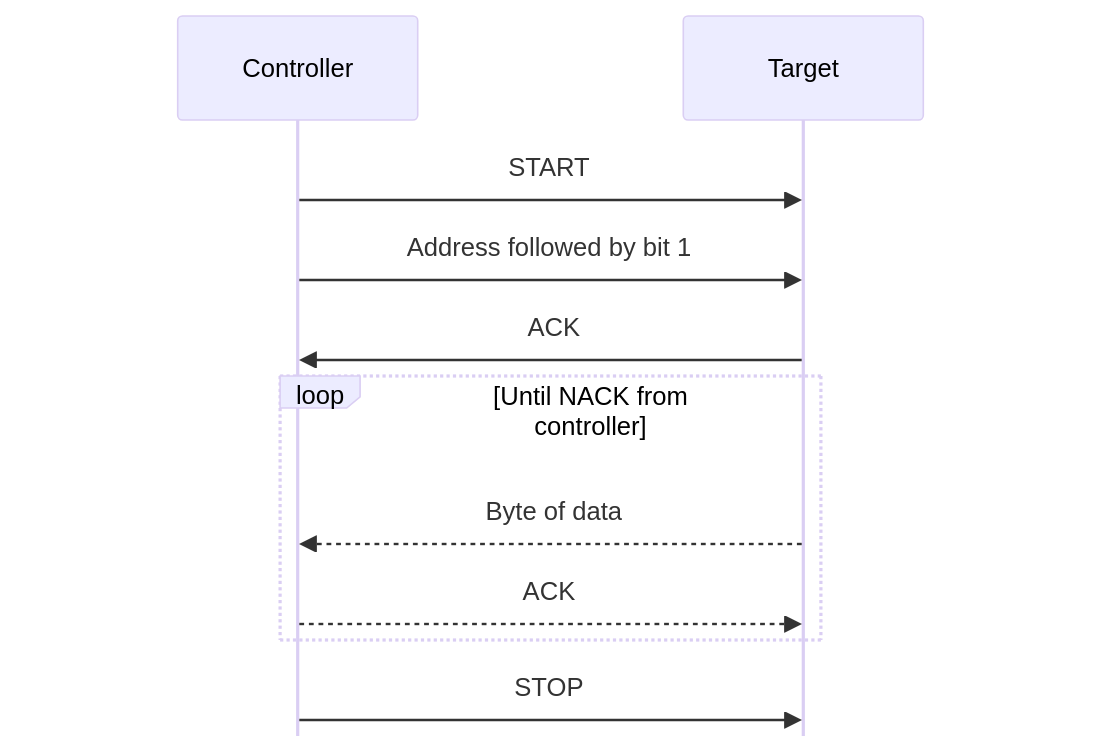
\includegraphics[width=0.5\textwidth]{figures/read_example.png}
    \caption{Example sequence of a read operation.}
    \label{fig:read_example}
\end{figure}

Further communication is performed by one party sending data, most significant bit first, and the other sending an \gls{ACK} bit.

\subsubsection{Bus sharing}

In the case of multiple targets linked with one controller, the controller needs to indicate which target it wants to interact with. To achieve this, each target compares the address sent by the controller with its own. If the address matches, it sends a low voltage \gls{ACK} bit back to the controller. If the address doesn't match, the target does nothing and the \gls{SDA} line remains high.

When there are multiple controllers, issues can arise, precisely when they try to send or receive data at the same time over the \gls{SDA} line. To solve this problem, each controller needs to detect if the \gls{SDA} line is low or high before transmitting a message. If the \gls{SDA} line is low, another controller is in control of the bus, and it should wait until a STOP has been received to send the message. If the \gls{SDA} line is high, then it's safe to transmit the message.

\subsubsection{Methods}
\label{sec:methods}

The protocol defines three basic types:
\begin{itemize}
    \item Write: Controller writes bytes to the target.
    \item Read: Controller reads bytes from the target until a given buffer is full.
    \item Write-read: Controller first writes bytes and then reads enough bytes to fill the buffer in a single transaction.
\end{itemize}

It is also possible to combine a list of write and read operations inside a transaction contract.
Figure \ref{fig:read_example} showcases more in detail how a read operation works.

\subsection{SMBus}
% [het idee is dat er hier uitgelegd gaat worden van wat SMBus is en de relatie met I2C]

The \gls{SMBus}~\cite{smbus} is a subset derived from \gls{I2C} by Intel. Its main application is to monitor critical parameters on PC motherboards and in embedded systems. On the surface they are quite similar, but there are some subtle differences worth mentioning. For one, \gls{SMBus} will time out when \gls{SCL} is held low for more than 35 milliseconds. \gls{I2C} doesn't have an established timeout value, implicating that a target or controller can hold \gls{SCL} as long as necessary to process data. \\
On account of this timeout, \gls{SMBus} has a minimum clock speed of 10 kHz. Leading to a maximum of 100 kHz. As stated earlier, \gls{I2C} can go as fast as 5 Mbit/s and no minimum frequency is specified.

Another difference is in terms of voltage levels. For \gls{I2C} the typical levels are +5 V, +3.3 V or even +1.8 V and below. In contrast, in an \gls{SMBus} system the supply ranges are restricted between +1.8 V and +5 V. In general, even with the different specifications for the input logic voltage thresholds, \gls{I2C} and \gls{SMBus} devices will be interoperable over the supply voltages permitted by the SMBus specification.

Sometimes libraries that provide methods for \gls{I2C} communication, also provide ones for \gls{SMBus}. But, thus, in the context of driving an \gls{I2C} target device, these can be safely ignored.


\clearpage
\section{Interfacing hardware}
\label{sec:hardware}
% [Deze sectie draait rond HAL, wat het is, waarom het nodig is en waarom het nuttig is om een gelijkaardige API te voorzien. Ter inspiratie kan de \verb|embedded_hal| scope en design goals genomen worden.]

Embedded devices have a high degree of diversity of possible constraints, e.g. 64-bit support, memory size and the availability of hardware units like a memory protection unit. Making it difficult for drivers to support any number of target platforms, unless these platforms are abstracted away behind a shared API. This is the purpose of a \gls{HAL}. It is important that this layer hides device-specific details and that it is generic across devices. 

For Rust, this \gls{HAL} is, aptly, named \texttt{embedded-hal}~\cite{gh:eh} and provides traits for using peripherals commonly available in microcontrollers such as \gls{GPIO}, \gls{UART}, \gls{SPI} or \gls{I2C}. There exists many crates that implement these interfaces for a certain microcontroller family or a system running some \gls{OS}. Furthermore, there are also loads of driver crates that use the \texttt{embedded-hal} interface to support all these families and systems. A curated list can be found in the Awesome Embedded Rust~\cite{gh:aer} repository.

Sadly, the notion of a community-wide shared interface is not universally present in all embedded communities. The C/C++ community is such an example, where there isn't one \gls{HAL} to rule them all.

\subsection{Different versions of \texttt{embedded-hal}}

Unfortunately, there are two major versions of \texttt{embedded-hal}, i.e. 0.2.7 and 1.0, which are incompatible with one another. 
As version 1.0 was only released on the ninth of January 2024, it is still fairly novel. Thus, crates have a wildly varying degree of compliance with this version. 

Broadly speaking, there are four major changes \cite{hal:1}. Firstly, traits have been simplified and others have been merged to remove interopability gotchas. 
Secondly, async versions of the blocking traits are now available in the \texttt{embedded-hal-async} crate. Thirdly, there is now support for \gls{SPI} bus sharing. Lastly and fourthly, there is improved error handling.

There is a crate~\cite{gh:ehcl} that tries to provide a compatibility layer between these two versions, but the latest supported version is merely a release candidate of 1.0. Thus, the crate is not really practically useful.

\subsection{Peripheral Access Crates}

\gls{SVD} files are \texttt{XML} files typically provided by silicon vendors which descibe the memory map of a device. Via the \texttt{svd2rust} crate~\cite{crates:svd2rust} it is possible to generate a mostly-safe Rust wrapper. Further discussion is out of scope as this is a very thin wrapper, and usually depended upon by \gls{HAL} authors.

\subsection{Running the solution}
\label{sec:running}

When the target platform is an \gls{OS}, it is typically fairly easy to build and execute a software solution, plainly by doing this on the target device itself, or by cross-compilation from a morepotent device. This is not the case for an \gls{MCU}, here, only cross-compilation is possible. Due to the constrained nature of memory on an \gls{MCU}, the memory-layout also needs to be specified.

In the case of a Raspberry Pi Pico, compilation results in an \texttt{UF2} and an \texttt{ELF} file. The former is a file format developed by Microsoft for flashing microcontrollers over mass storage connections. The latter is used by the debugger.

To pogram the flash on the Pico, the \texttt{BOOTSEL} button needs to be held, forcing it into USB Mass Storage Mode. Then, you can move a \texttt{UF2} file onto it. Whereupon the \texttt{RP2040} processor of the Pico will reboot, unmount itself, and run the flashed code. Other boards could require pulling down the flash \texttt{CS} pin, which is how the \texttt{BOOTSEL} button works on the pico, using an exposed \gls{SWD} interface, also an option for the Pico, or have a reset button that needs to be double-pressed.

\gls{SWD} is a standard interface on Cortex-M based microcontrollers, which the host machine can use to reset the board, load code into flash, and set the code running. Without the need to manually reset the board or hold the \texttt{BOOTSEL} button. The easiest way to connect with this interface on a Pico is to make use of a debug probe via \texttt{probe-rs}~\cite{probe-rs}. This also unlocks the ability to print to \texttt{STDOUT} or even utilize the Debug Adapter Protocol~\cite{dap}.


\clearpage



% Vanaf hier mag er geen nieuwe kennis meer geïntroduceerd worden!
\chapter{Architecture and standard}
\label{chap:architecture}
% [Vertellen over de proposal, hoe championship werkt, wat de huidige status is en wat er moet gedaan worden om het te advancen. Daarnaast ook de laatste status rond SIG Embedded vertellen en de missie ervan.]

% 1. Primer om te vertellen wat nodig is om dan de rest te snappen

Currently, the \gls{I2C} proposal~\cite{gh:i2c} is in the second phase, with ongoing effort to fullfill the criteria to pass the vote to the third phase. Specifically, the following requirements are yet to be met:

\begin{itemize}
    \item The proposal lacks a test suite that covers the feature.
    \item Some pull requests and issues are still open that iterate on the design of the feature.
    \item Updates to the reference interpreter are not yet required, but recommended.
\end{itemize}

This effort is led under the guidance of certain champions, for this proposal these are Friedrich Vandenberghe, Merlijn Sebrechts and Maximilian Seidler. Both Friedrich and Merlijn are from UGent, Maximilian is from Siemens. This mix of academians and people from the industry ensures ongoing standardization effort and actual usage of the feature.

At the start of this thesis \texttt{wasi-i2c} was merely an idea, lacking any proposal or implementation, and thus technically, still residing in phase zero. But now it contains three \gls{WIT} files that follow the component model: \texttt{delay}, \texttt{i2c} and \texttt{world}. The first two closely follow the corresponding interfaces from \texttt{embedded-hal} version 1, \texttt{embedded-hal} is explained in section~\ref{sec:hardware}, but this crate is not necessary for an implementation. The philosphy behind this is the same as for why one would want to have an \texttt{embedded-hal}.

\begin{listing}[h]
\begin{minted}[samepage]{rust}
package wasi:i2c@0.2.0-draft;

world imports {
    import i2c;
    import delay;
}
\end{minted}
\caption{The \texttt{world.wit} file inside the \texttt{wasi-i2c} proposal.}
\label{code:world}
\end{listing}

The proposal defines two handles, for an explainer on handles see~\ref{sec:design}, one for \gls{I2C} and one for delays. These provide pretty broad access, e.g. it is not possible to limit the \gls{I2C} connection to certain addresses. A more fine-grained control model is possible, but there's currently no demand for this.

Inside the \texttt{i2c} interface, no explicit constructor is defined because \texttt{i2c} resources can be constructed in many different ways, so worlds that include this interface should also include a way to obtain \gls{I2C} handles. Typically, this is done by either having handles passed into exported functions as parameters, or by having handles returned from imported functions.
The definition for \texttt{world.wit} can be found in codefragment~\ref{code:world}. The purpose of this world is to provide a way to import all the defined interfaces in the proposal at once.

Although delays are not inherently linked with \gls{I2C}, some guests implementations require this, and thus it is part of the proposal. In the future, it could be that delays get split up into their own proposal, or that this proposal gets merged with the other embedded-related proposals. The biggest drawback to a merger would be that this, possibly, could heavily increase the burden on the champions. Furthermore, this would require that all the champions are interested in maintaining all of these other communication protocols. On the other hand, this would centralize the proposals and could make it easier for potential implementors.

\section{Asynchronous I2C}

Currently, the proposal is purely synchronous. To provide an asynchronous (async) API, there are two possible ways to tackle this:

\begin{description}
    \item[Explicit] A seperate WIT API could be provided that depends on \texttt{wasi-io}~\cite{gh:io} polling. This could be implemented with the current tooling.
    \item[Integrated] Wait for the Component Model to natively integrate async. The major upside to this approach is that a single WIT description can describe both a sync and async API. Caller and callee can each independently choose if they want to be sync or async, and they can be linked.
\end{description}

As there's no immediate need for this, the champions have decided that it is best to wait until the integrated option is mainstream.

\newpage

\section{Portability criteria}

An important part of a proposal is its portability criteria, with these the champions show that their specification isn't overspecified for a specific platform. Commonly, these are two complete independent implementations, but due to the diversity in platforms that can interact with I2C this isn't suitable for the \texttt{wasi-i2c} proposal. 

\begin{table}[h]
	\centering
	\captionsetup{justification=centering}
	\begin{tabular}{c c l}
		\toprule
		Platform & Architecture & Reference hardware \\ \midrule
        Linux    & ARM64 & Raspberry Pi 3 Model B \\
        RTOS    & RISC-V & ESP32-C2 \\
        RTOS      & ARM32 & Nucleo F412ZG \\
		\bottomrule
	\end{tabular}
    \caption{\texttt{wasi-i2c} portability criteria}
	\label{tab:criteria}
\end{table}

The champions, together with people from Siemens, Intel, Aptiv, Xiaomi, Amazon, Midokura, Sony, Atym and Bosch, have agreed upon a set of criteria for the proposal. These criteria can be found in Table~\ref{tab:criteria}. For each criterium, reference hardware is provided, without these there would still be a lot of possible variety in RAM size, flash size and CPU speed. Herein Intel x86 is missing, but support for this is implied as this is the used architecture for developing Wasmtime. The Nucleo is chosen because this is the reference board for Siemens. The other two are chosen to showcase support for both RTOS and Linux, and ARM and RISC-V.
As an extra requirement besides the targets, it is important that the interface is designed in such a way that memory usage is limited to the bare needed minimum, to ensure enough RAM left for the application itself.


\chapter{Implementations}
\label{chap:implementation}
% [De hele hardware setup uitleggen, dus de verschillende Pi's en de apparaten waar er mee gepraat wordt.]
As stated in chapter~\ref{chap:architecture}, it is necessary to provide implementations to ascertain the soundness of the \gls{WIT} interfaces. Ideally, these are as diverse as possible. Both in terms of operations on the \gls{I2C} connection, and the target architectures.

Three implementations are provided: one that performs an \gls{I2C} read and two that write to an \gls{I2C} connection, developed for three devices targeting two architectures. 
On the one hand, we have a Raspberry Pi 3 and 4 targeting ARM64 Linux, and on the other hand we have a Raspberry Pi Pico \gls{MCU} targeting RP2040 processor.

% TODO: DHT22 en ESP8266 opzoeken
On the Pi 3, a \gls{HAT} is mounted that contains a HTS221 sensor, from which the current temperature and humidity is read. The Pi 4 is either connected with a HD44780 LCD character display or a 4-digit 7-segment display. 
Although the Pi 3 could also be linked up with these displays, it's more of a hassle thanks to the \gls{HAT}. The pico is solely linked with the 4-digit display. Because of the \gls{MCU} constraints, controlling the HD44780 is out of scope.

\begin{figure}[h]
    \centering
    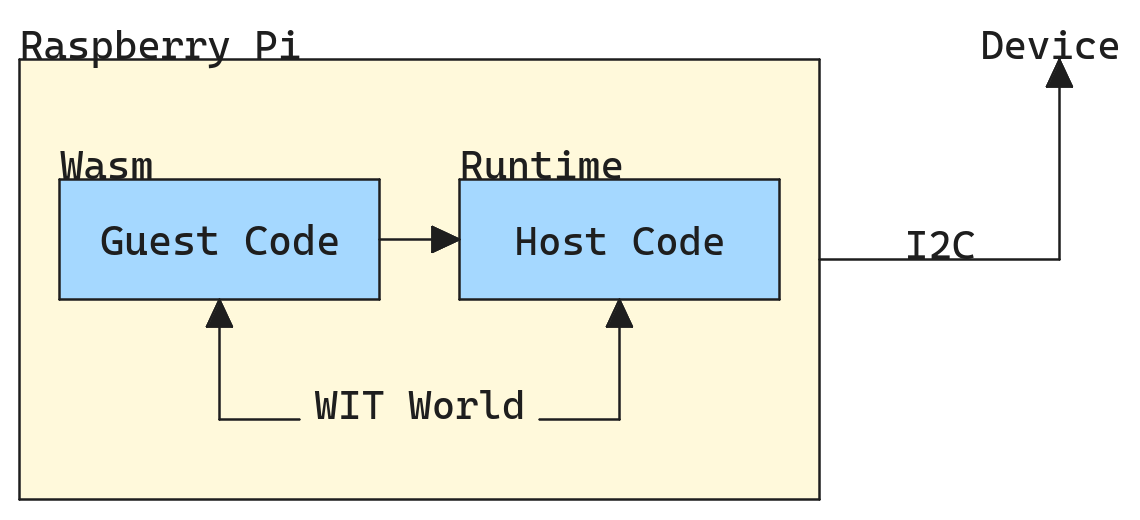
\includegraphics[width=0.5\textwidth]{figures/schema.png}
    \caption{Schematic overview of an implementation.}
    \label{fig:schematic}
\end{figure}

Conceptually, each implementation comes down to the schematic defined in figure~\ref{fig:schematic}. Only the guest code differs for each device. See chapter~\ref{chap:wasm} for an in-depth explanation.

% TODO: Hier foto's zetten van de verschillende setups

\section{Embedded driver development in Rust}
% [Native driver development, hoe gaat het te werk en de grote verschillen voor native development voor een gewone Pi en een microcontroller zoals de Pi Pico.]
Besides the implementation itself, two things are of significance to design a device driver in Rust. Namely, following the Embedded \gls{HAL} \gls{API}, see chapter~\ref{chap:hardware}, and supporting the desired target architecture.

Fortunately, Rust provides support for a great deal of platforms. Thus, building for ARM64 is as simple as providing the \texttt{--target aarch64-unknown-linux-gnu} flag. However, the RP2040 architecture needs special attention. For this, besides setting the \texttt{--target} flag with \texttt{thumbv6m-none-eabi}, we also need to provide a file called \texttt{memory.x}. 
This file is a linker script which specifies the memory layout of the target device, see section~\ref{sec:running}. Furthermore, the \gls{MCU} has only support for a \texttt{no\_std}.

\section{Embedded driver development in WebAssembly}
% [Om van native naar Wasm te gaan, wat moet er veranderen.]embedded-hal 0.2 vs 1.0 vermelden
Besides the considerations from the previous section, we now also need to keep the used runtime target platform support in mind. See section~\ref{sec:runtimes} for an overview. Furthermore, in this section, the different features of each runtime are also highlighted. These led to a vastly different implementation for both the host and the guest code.

\subsection{Wasmtime}

The guest is made into a component via the procedure specified in section~\ref{sec:guest}. The configured \gls{WIT} interface is the one specified in codefragment~\ref{code:wit}. 
Herein \texttt{wasi:i2c} is the proposal, as explained in chapter~\ref{chap:architecture}. Both displays are represented by the \texttt{screen} world, which needs both \texttt{i2c} and \texttt{delay} from the proposal. The HTS221 is mapped with the \texttt{sensor} world, that only needs \texttt{i2c}. Therefore, the former just includes the imports from \texttt{wasi:i2c}, while the latter only imports \texttt{i2c}.

The generated bindings have no way of knowing that they actually should follow the \texttt{embedded-hal} traits, for this the \href{https://github.com/Zelzahn/wasi-embedded-hal}{wasi-embedded-hal} crate is used.

On the side of the host, binding is done as described in section~\ref{sec:host}. Here, \texttt{wasi:i2c} is seen as a missing import, thus the \texttt{with} option is used with a data structure that implements the necessary traits.

\begin{listing}[h]
\begin{minted}[samepage]{rust}
package sketch:implementation;

interface hts {
    use wasi:i2c/i2c@0.2.0-draft.{i2c, error-code};

    get-temperature: func(connection: i2c) -> result<string, error-code>;
    get-humidity: func(connection: i2c) -> result<string, error-code>;
}

interface lcd {
    use wasi:i2c/i2c@0.2.0-draft.{i2c};
    use wasi:i2c/delay@0.2.0-draft.{delay};

    write: func(connection: i2c, delay: delay, message: string);
}

world sensor {
    import wasi:i2c/i2c@0.2.0-draft;

    export hts;
}

world screen {
    include wasi:i2c/imports@0.2.0-draft;

    export lcd;
}
\end{minted}
\caption{The \gls{WIT} interface to which guest and host bind.}
\label{code:wit}
\end{listing}

\subsection{WAMR}
% [vertellen dat ik in WAMR constrained was tot het doorgeven van simpele datatypes en dan maar met die globale connectie gewerkt heb]
As explained in section~\ref{sec:runtimes}, \gls{WAMR} is a lightweight runtime that, currently, has no support for preview 2. To sustain a pure Rust codebase, \href{https://github.com/bytecodealliance/wamr-rust-sdk}{WAMR Rust SDK} is used. This SDK provides Rust language bindings and support for passing integers and floats between the host and the guest. Note that strings can be passed via a conversion to a vector of the string code points.

As we can no longer use \gls{WIT}, nor pass a connection to the guest, we are enforced to greatly differ from the Wasmtime implementation. Therefore, we will focus us on the simpler 4-digit 7-segment display with the following conceptuel differences for \gls{WAMR}: The \gls{I2C} connection is kept global inside the host and there are now 4 arguments for the \texttt{write} function, one for each digit.

\subsection{Problems}
%TODO: Vertellen over gemerkte tekortkomingen aan WAMR, component model enzo
% Bvb. Is het mogelijk om Component Model voor MCU's te gebruiken

\chapter{Evaluation}
\label{chap:evaluation}

% [Benchmarks tonen en bespreken van het lezen van de temperatuur native vs in Wasm. Het is niet de bedoeling om de runtimes te benchmarken.]

% Kunnen het zien als een tweeluik:
% 1. Functionele evaluatie: Werkt het?
% 2. Niet-functionele evaluatie: Performantie

% Dit kan op twee manieren gestructureerd worden:
% - Per implementatie zeggen of het werkt en performant is
% - Eerst werkt het, alle setups overlopen en dan overzichtsgrafiekje geven
% 	- Deze manier heeft Merlijns voorkeur omdat je zo mooi meer meta kunt gaan

\section{Evaluation setup}

The evaluation setup is based upon the setups used for the implementations, as shown in Chapter~\ref{chap:implementation}. It consists of the following:

\begin{itemize}
  \item A Raspberry Pi 4 Model B with 8 GB of RAM hooked up with a 4-digit 7-segment LED
  \item A Raspbery Pi 3 Model B with an attached HTS221 sensor
\end{itemize}

The display is evaluated natively and with Wasmtime and \gls{WAMR} as a runtime. The sensor will be evaluated in the same manner, but without the WAMR runtime.

The execution time is measured with the \texttt{criterion.rs} crate~\cite{gh:criterion}. This crate performs a hundred measurements, each containing many iterations of a routine, and then accumulates this into a probability density function. It indicates the estimated probability of an iteration taking a certain amount of time. Furthermore, the plot also contains a vertical line, this indicates the mean execution time. Thanks to the immense range of factors that can influence the execution time, outliers will always occur, and the resulting density functions aren't set in stone. Due to these outliers, sometimes a smaller extra peak can appear. Before measuring, criterion first performs a warmup phase. Here, the routine is executed repeatdly to give the system time to adapt to the new workload. This helps prevent things like cold caches.

For memory profiling, \texttt{dhat-rs}~\cite{gh:dhat} is used. The profiler makes use of a global allocator that tracks allocations and deallocations on the heap. After execution, the total number of bytes, the maximum amount and the size at the end is printed. Together with the number of allocations.

The \texttt{flamegraph} crate~\cite{gh:flamegraph} is used to provide an in-depth overview of the functions an implementation uses under the hood. This overview is provided in fashion of flamegraphs. Many times per second, the threads in a program are interrupted and the current location in the code is recorded, along with the chain of functions that were called to get there. These samples are then processed and stacks that share common functions are added together. Then a figure is generated showing the call stacks that were measured. The x-axis doesn't show the passing of time. The left to right ordering has no meaning. The width of each block shows the total time that that function is on the CPU. A wider block means that it consumes more CPU per execution than other functions, or that it's called more. Each block's color is chosen at random.

\section{Functional evaluation}

This dissertation evaluates the applications on their execution time and used memory compared between running natively versus inside the Wasmtime and \gls{WAMR} runtimes. 

For this, two scenarios are tested:

\begin{itemize}
  \item On the Raspberry Pi 3 the temperature gets read out. This value is manually verified with the native implementation.
  \item On the Raspberry Pi 4 the string \texttt{"1234"} gets written to the display. This is visually verified, see Figure~\ref{fig:verif}.
\end{itemize}

\begin{figure}[h]
  \centering
  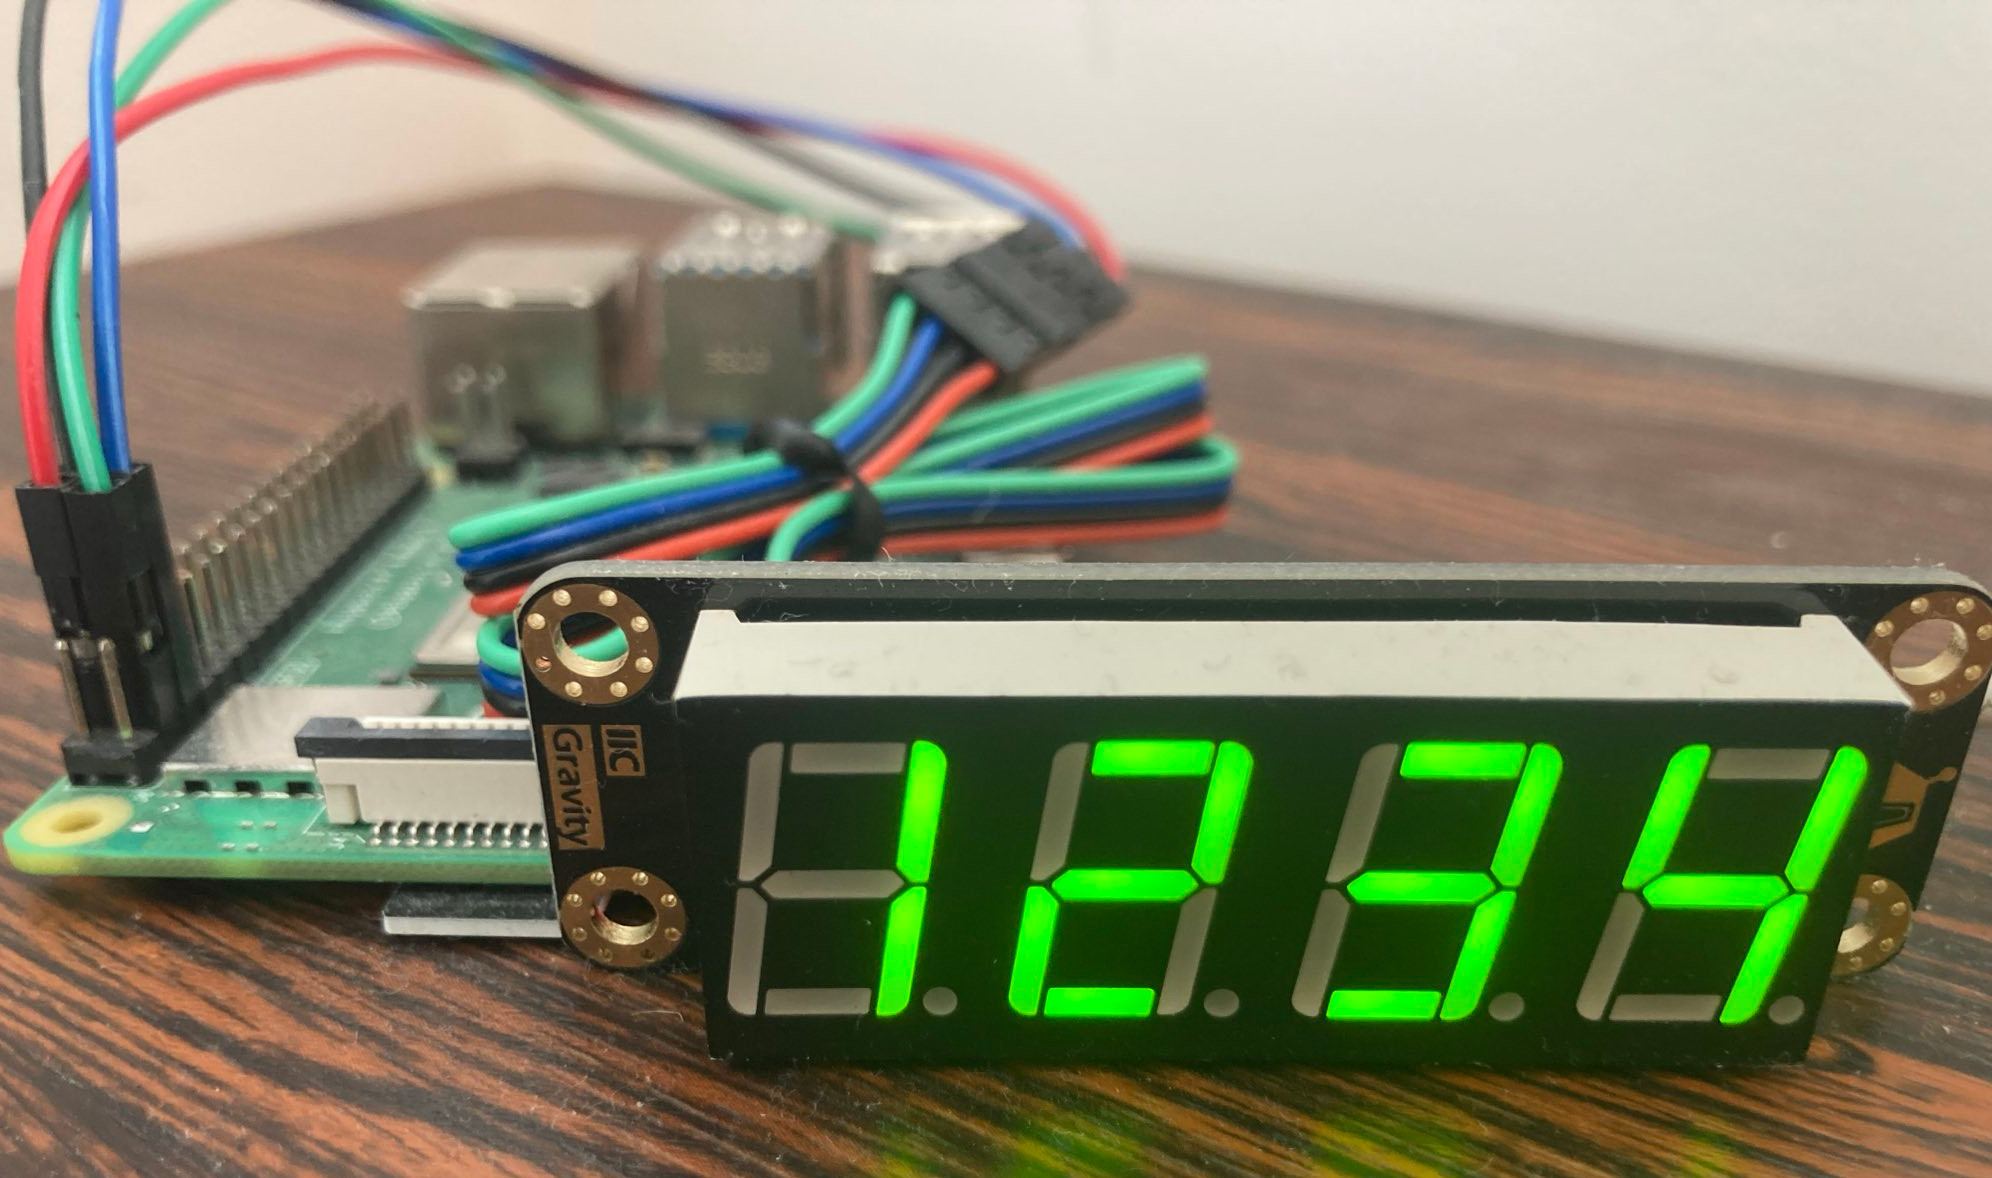
\includegraphics[width=0.5\textwidth]{figures/verification}
  \caption{Visual verification of the display}
  \label{fig:verif}
\end{figure}

\section{Benchmarks}

\begin{figure}[h]
  \centering
  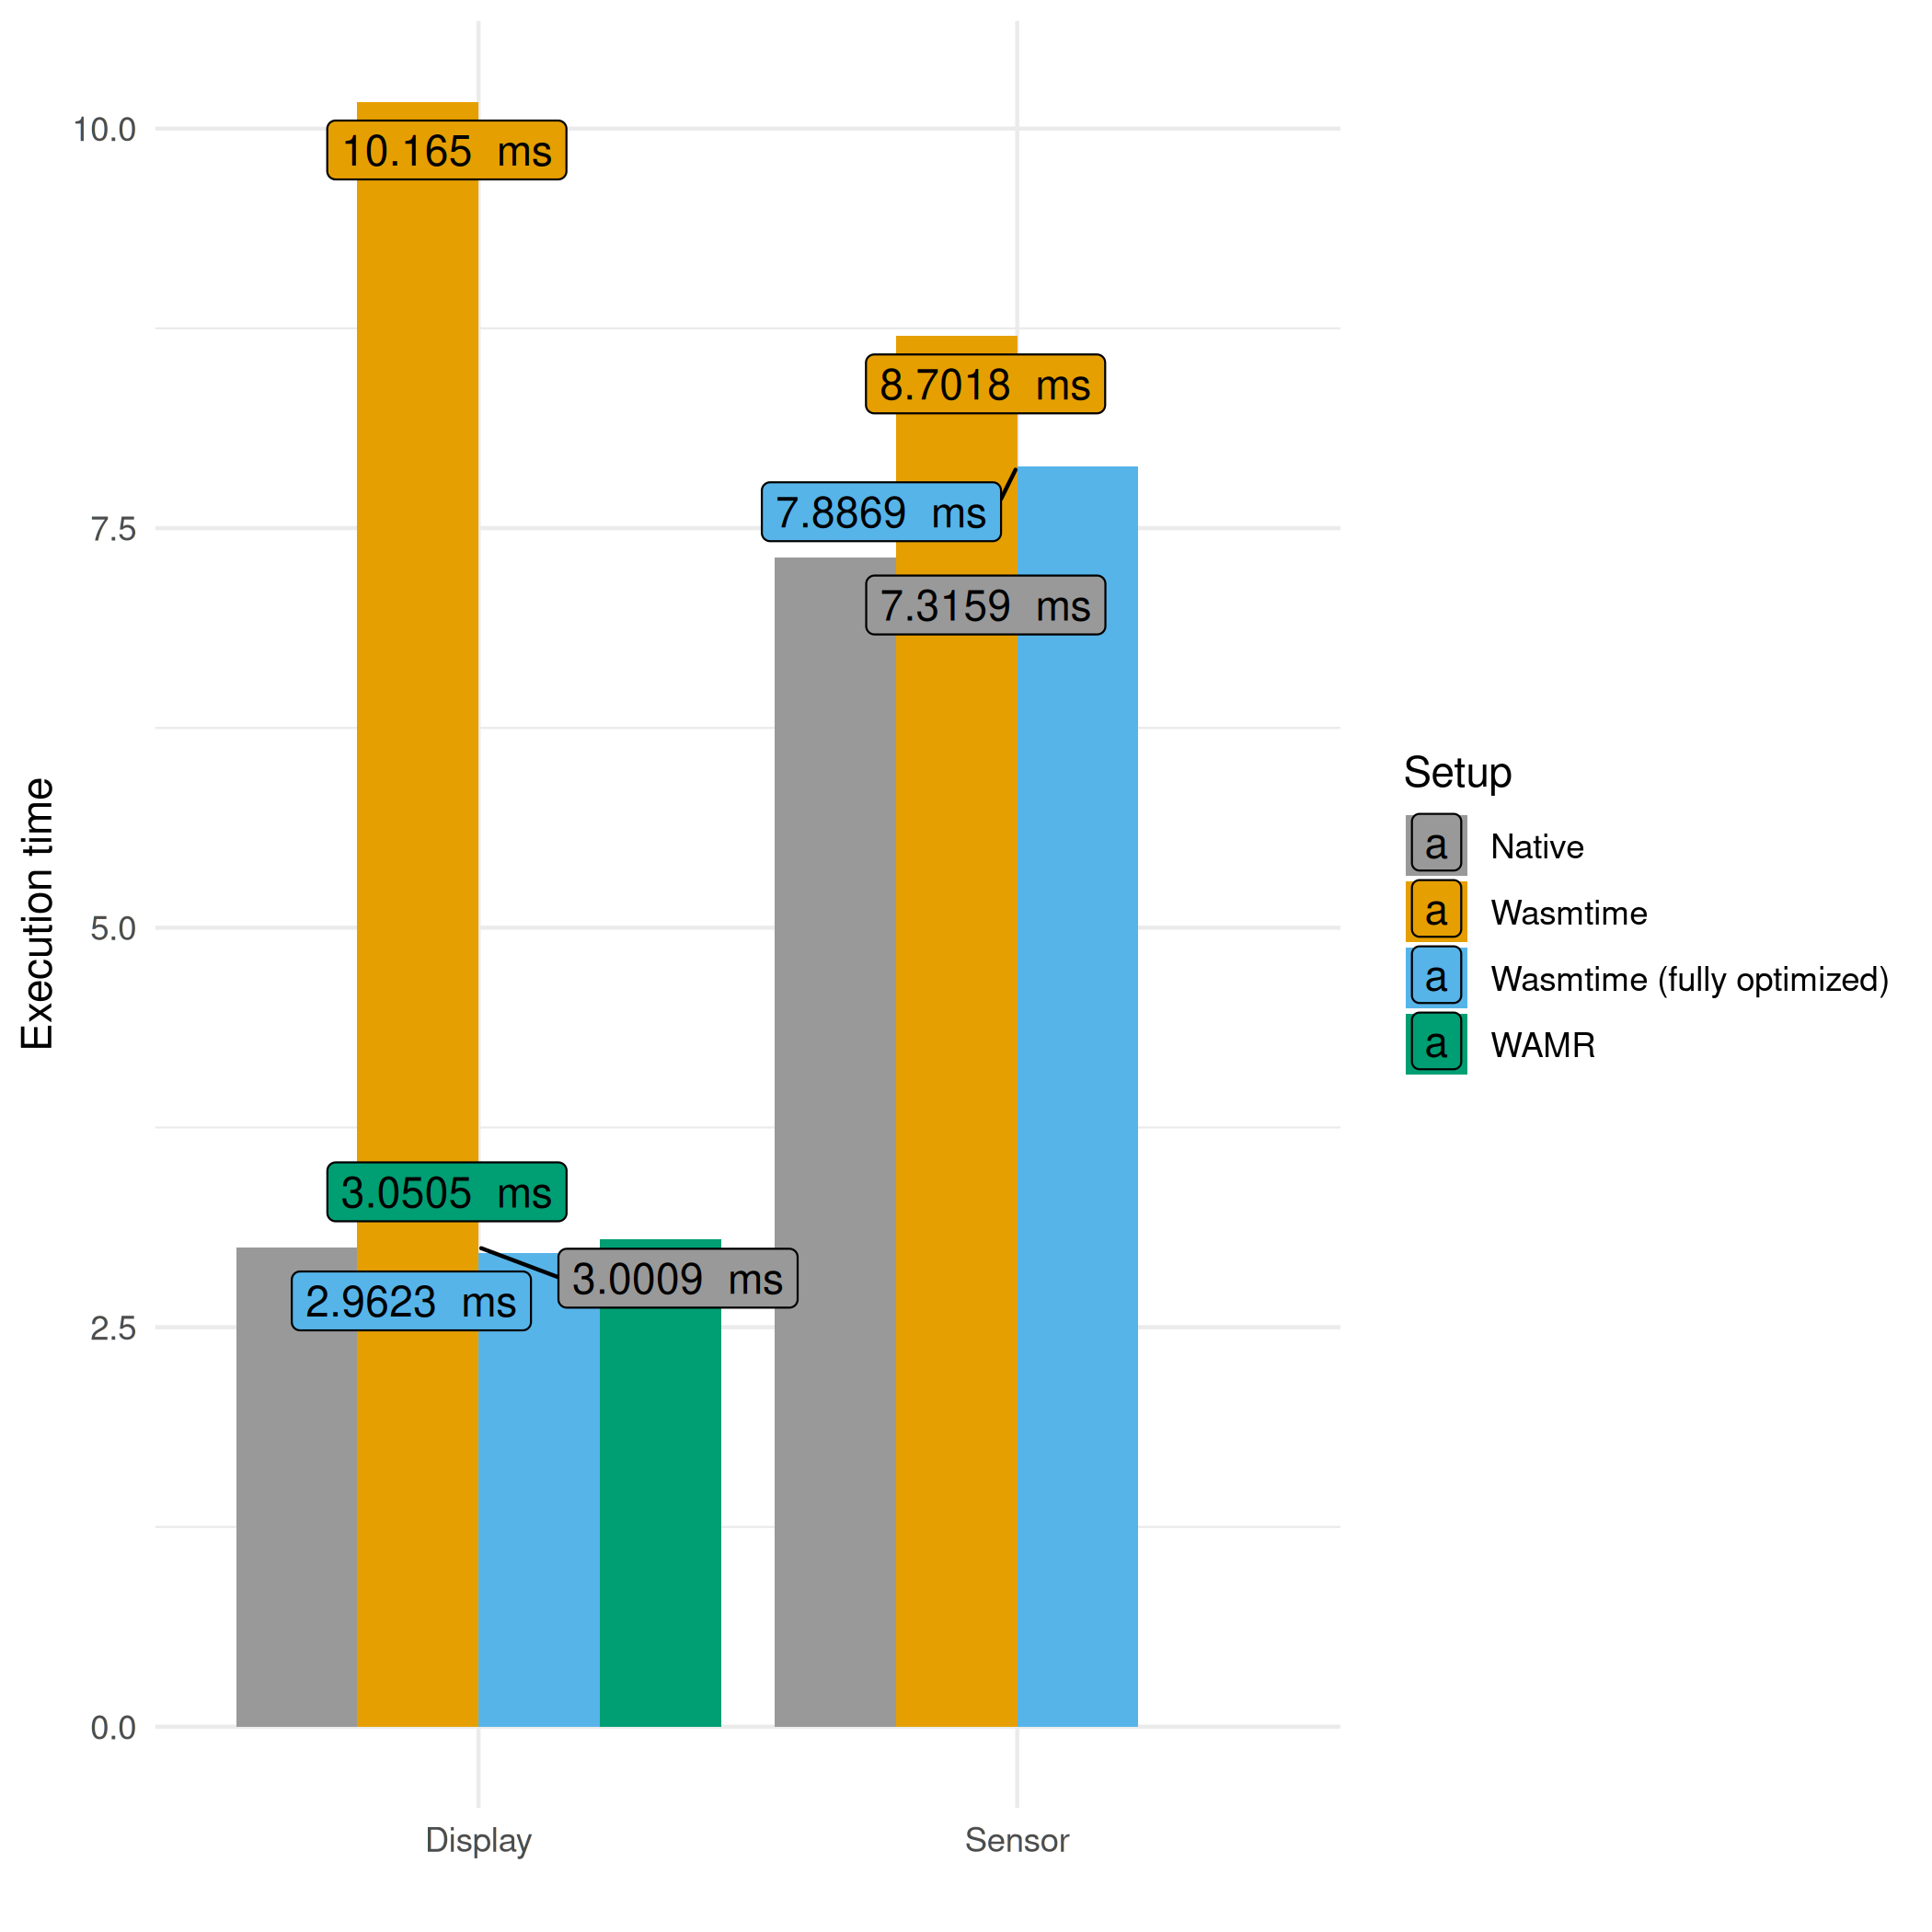
\includegraphics[width=.5\textwidth]{figures/execution_times}
  \caption{Overview of all the mean execution times}
  \label{fig:all:times}
\end{figure}

It is expected that running in Wasmtime will perform worse due to the imposed overhead on both execution time and memory usage, but that this overhead will be negligible. For WAMR, an even slimmer overhead is expected.

First, the execution time is inspected. An overview is available in Figure~\ref{fig:all:times}.
Both Figure~\ref{fig:display} and Figure~\ref{fig:sensor} showcase an astonishing longer execution time when running inside Wasmtime. The flamegraph in Figure~\ref{fig:flamegraph:wasmtime} gives the probable explanation, namely writing to the display is done inside the \texttt{\_start} block, almost all the other blocks are related to Cranelift.

Bytecode Alliance's Cranelift is a compiler backend that is among others in use by Wasmtime for just-in-time and ahead-of-time compilation. Via its ahead-of-time functionality, it is possible to greatly reduce the average execution time. There are two options to make use of this, through \texttt{wasmtime compile} or the \path{Component::serialize} function inside Wasmtime. To load such a precompiled file, the \path{Component::deserialize_file} function needs to be used, instead of \path{Component::from_file}. This file contains native, non-portable binary code which will not work on a different architecture, and might not even work across different processor models within the same architecture. Thus, it is not feasible to distribute a precompiled \gls{Wasm} binary, instead of the \gls{Wasm} binary itself\footnote{Technically, it is possible, but this requires careful configuration and is too complex for this dissertation.}.

\begin{figure}[h]
\centering
\begin{subfigure}{.5\textwidth}
  \centering
  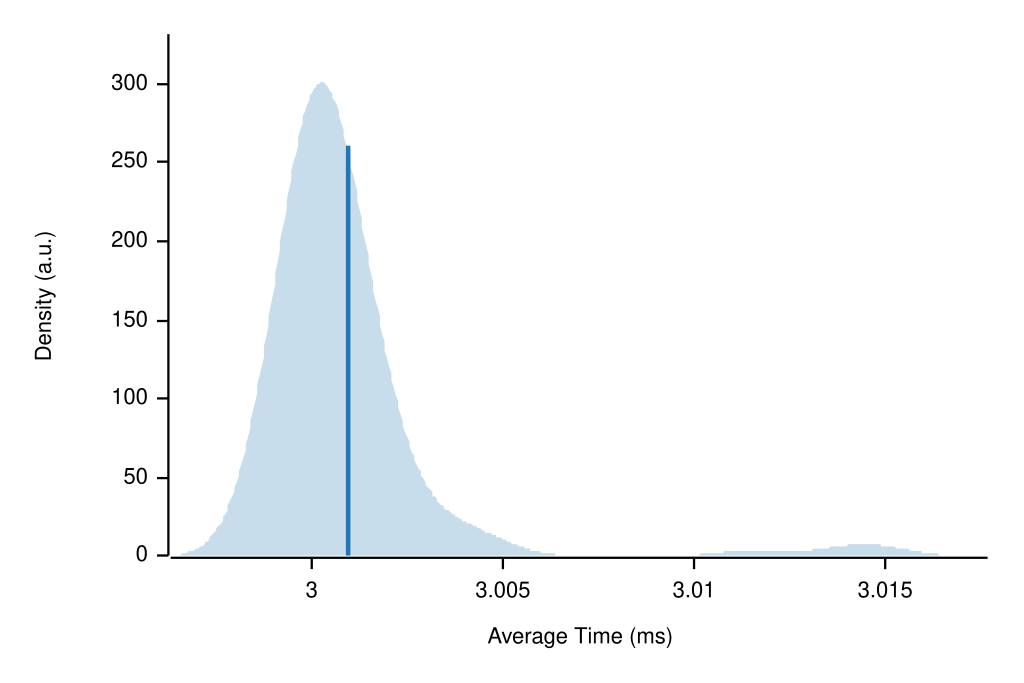
\includegraphics[width=\linewidth]{figures/native_led}
  \caption{Native}
  \label{fig:native_led}
\end{subfigure}%
\begin{subfigure}{.5\textwidth}
  \centering
  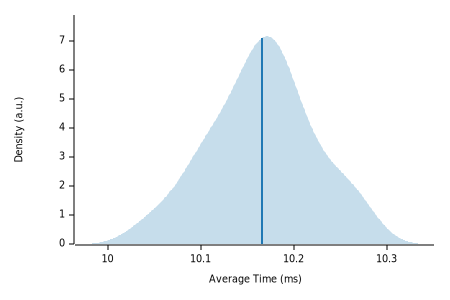
\includegraphics[width=\linewidth]{figures/wasmtime_led}
  \caption{Inside Wasmtime}
  \label{fig:wasmtime_led}
\end{subfigure}

\begin{subfigure}{.5\textwidth}
  \centering
  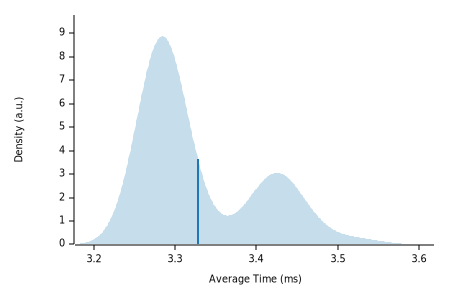
\includegraphics[width=\linewidth]{figures/compiled_led}
  \caption{Inside Wasmtime (precompiled)}
  \label{fig:led:compiled}
\end{subfigure}%
\begin{subfigure}{.5\textwidth}
  \centering
  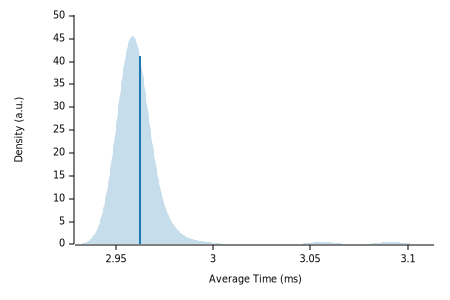
\includegraphics[width=\linewidth]{figures/optim_compiled_led}
  \caption{Inside Wasmtime (precompiled \& no command world)}
  \label{fig:led:wasmtime}
\end{subfigure}

\caption{Probability density function of execution time when writing to the display on....}
\label{fig:display}
\end{figure}

\begin{figure}[h]
\centering
\begin{subfigure}{.5\textwidth}
  \centering
  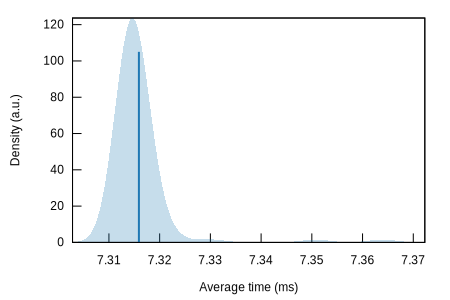
\includegraphics[width=\linewidth]{figures/native_hat_2}
  \caption{Native}
  \label{fig:native_hat}
\end{subfigure}%
\begin{subfigure}{.5\textwidth}
  \centering
  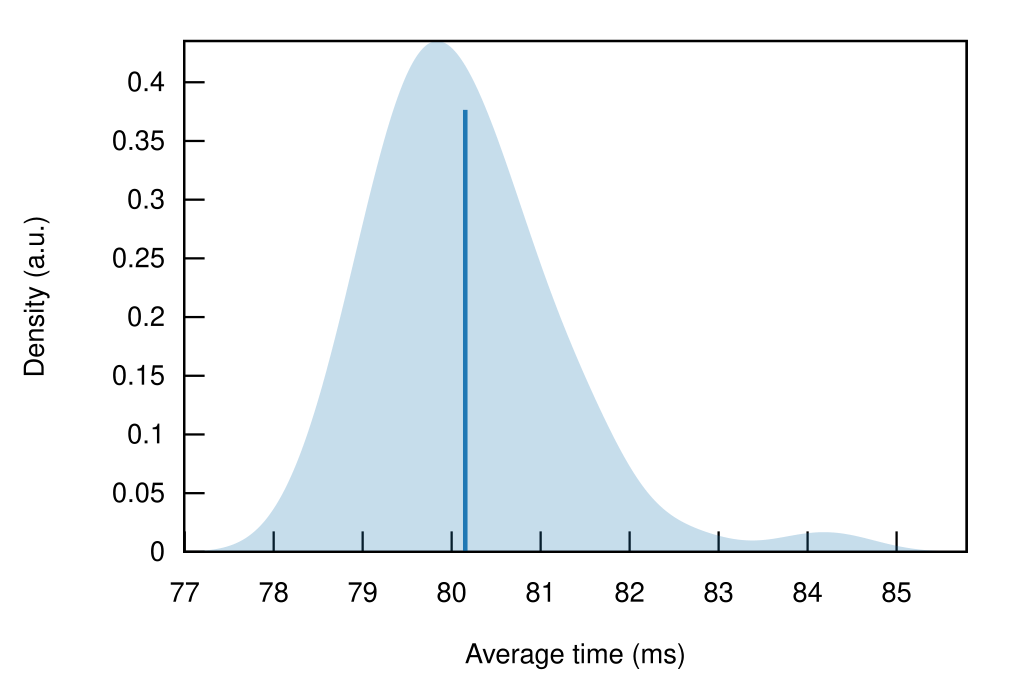
\includegraphics[width=\linewidth]{figures/wasmtime_hat}
  \caption{Inside Wasmtime}
  \label{fig:wasmtime_hat}
\end{subfigure}

\begin{subfigure}{.5\textwidth}
  \centering
  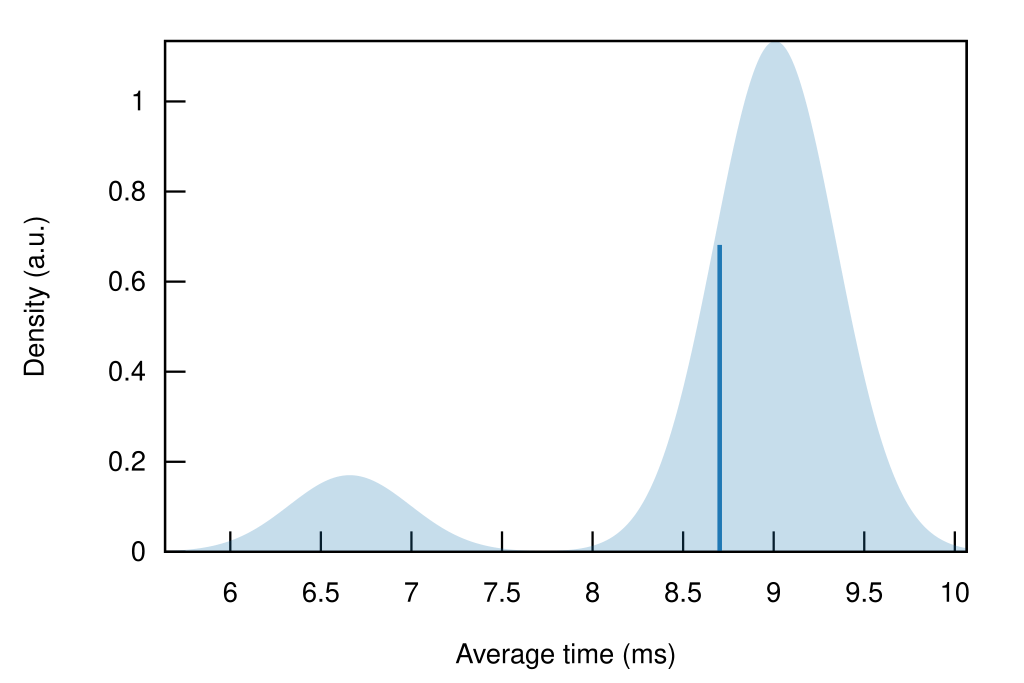
\includegraphics[width=\linewidth]{figures/compiled_hat}
  \caption{Inside Wasmtime (precompiled)}
  \label{fig:hat:compiled}
\end{subfigure}%
\begin{subfigure}{.5\textwidth}
  \centering
  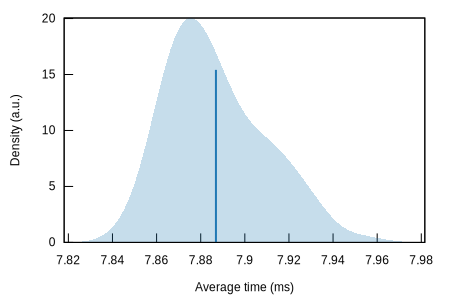
\includegraphics[width=\linewidth]{figures/optim_compiled_hat}
  \caption{Inside Wasmtime (precompiled \& no command world)}
  \label{fig:hat:wasmtime}
\end{subfigure}%

\caption{Probability density function of execution time when reading from the sensor on....}
\label{fig:sensor}
\end{figure}

Figure~\ref{fig:led:compiled} shows the execution time with a precompiled binary. It now is far more comparable to the average time of the native execution, with only an estimated slower mean run time of 0.3062 milliseconds. The same holds true for reading the sensor, Figure~\ref{fig:hat:compiled}, where the slowdown is now merely 1.3859 milliseconds. But, when compared to the experienced slowdown of the display implementation, this is still too much. The flamegraph inside Figure~\ref{fig:flamegraph:sensor} shows that nearly 14\% of the time is spent with adding the command world to the linker, using the \texttt{command::sync::add\_to\_linker} function, while this world technically isn't needed because of the custom host setup. Without this world, reading the sensor in Wasmtime is now only 0.571 milliseconds slower, Figure~\ref{fig:hat:wasmtime}, and writing to the display is 38.6 microseconds faster than native, Figure~\ref{fig:led:wasmtime}. The executed functions, see Figure~\ref{fig:flamegraph:led:native} and Figure~\ref{fig:flamegraph:led:compiled}, do not show any prominent differences. Thus, the speedup could be due to noise or kernel intrinsics.

\begin{figure}[h]
  \centering
  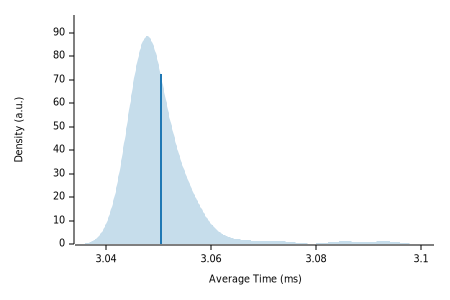
\includegraphics[width=0.5\textwidth]{figures/wamr_led}
  \caption{Execution time when writing to the display inside WAMR}
  \label{fig:led:wamr}
\end{figure}

\newpage

Comparing WAMR with the fastest Wasmtime version for writing to the display, thus Figure~\ref{fig:led:wamr} with \ref{fig:led:wasmtime}, shows that Wasmtime outperforms with 88.2 microseconds. This is not significant enough of a difference for one to be faster or slower than the other. Looking at the flamegraph for WAMR, Figure~\ref{fig:flamegraph:led:wamr}, it is apparant that a considerable amount of time is spent on a page translation fault. 

\begin{figure}[h]
\centering
\begin{subfigure}{.5\textwidth}
  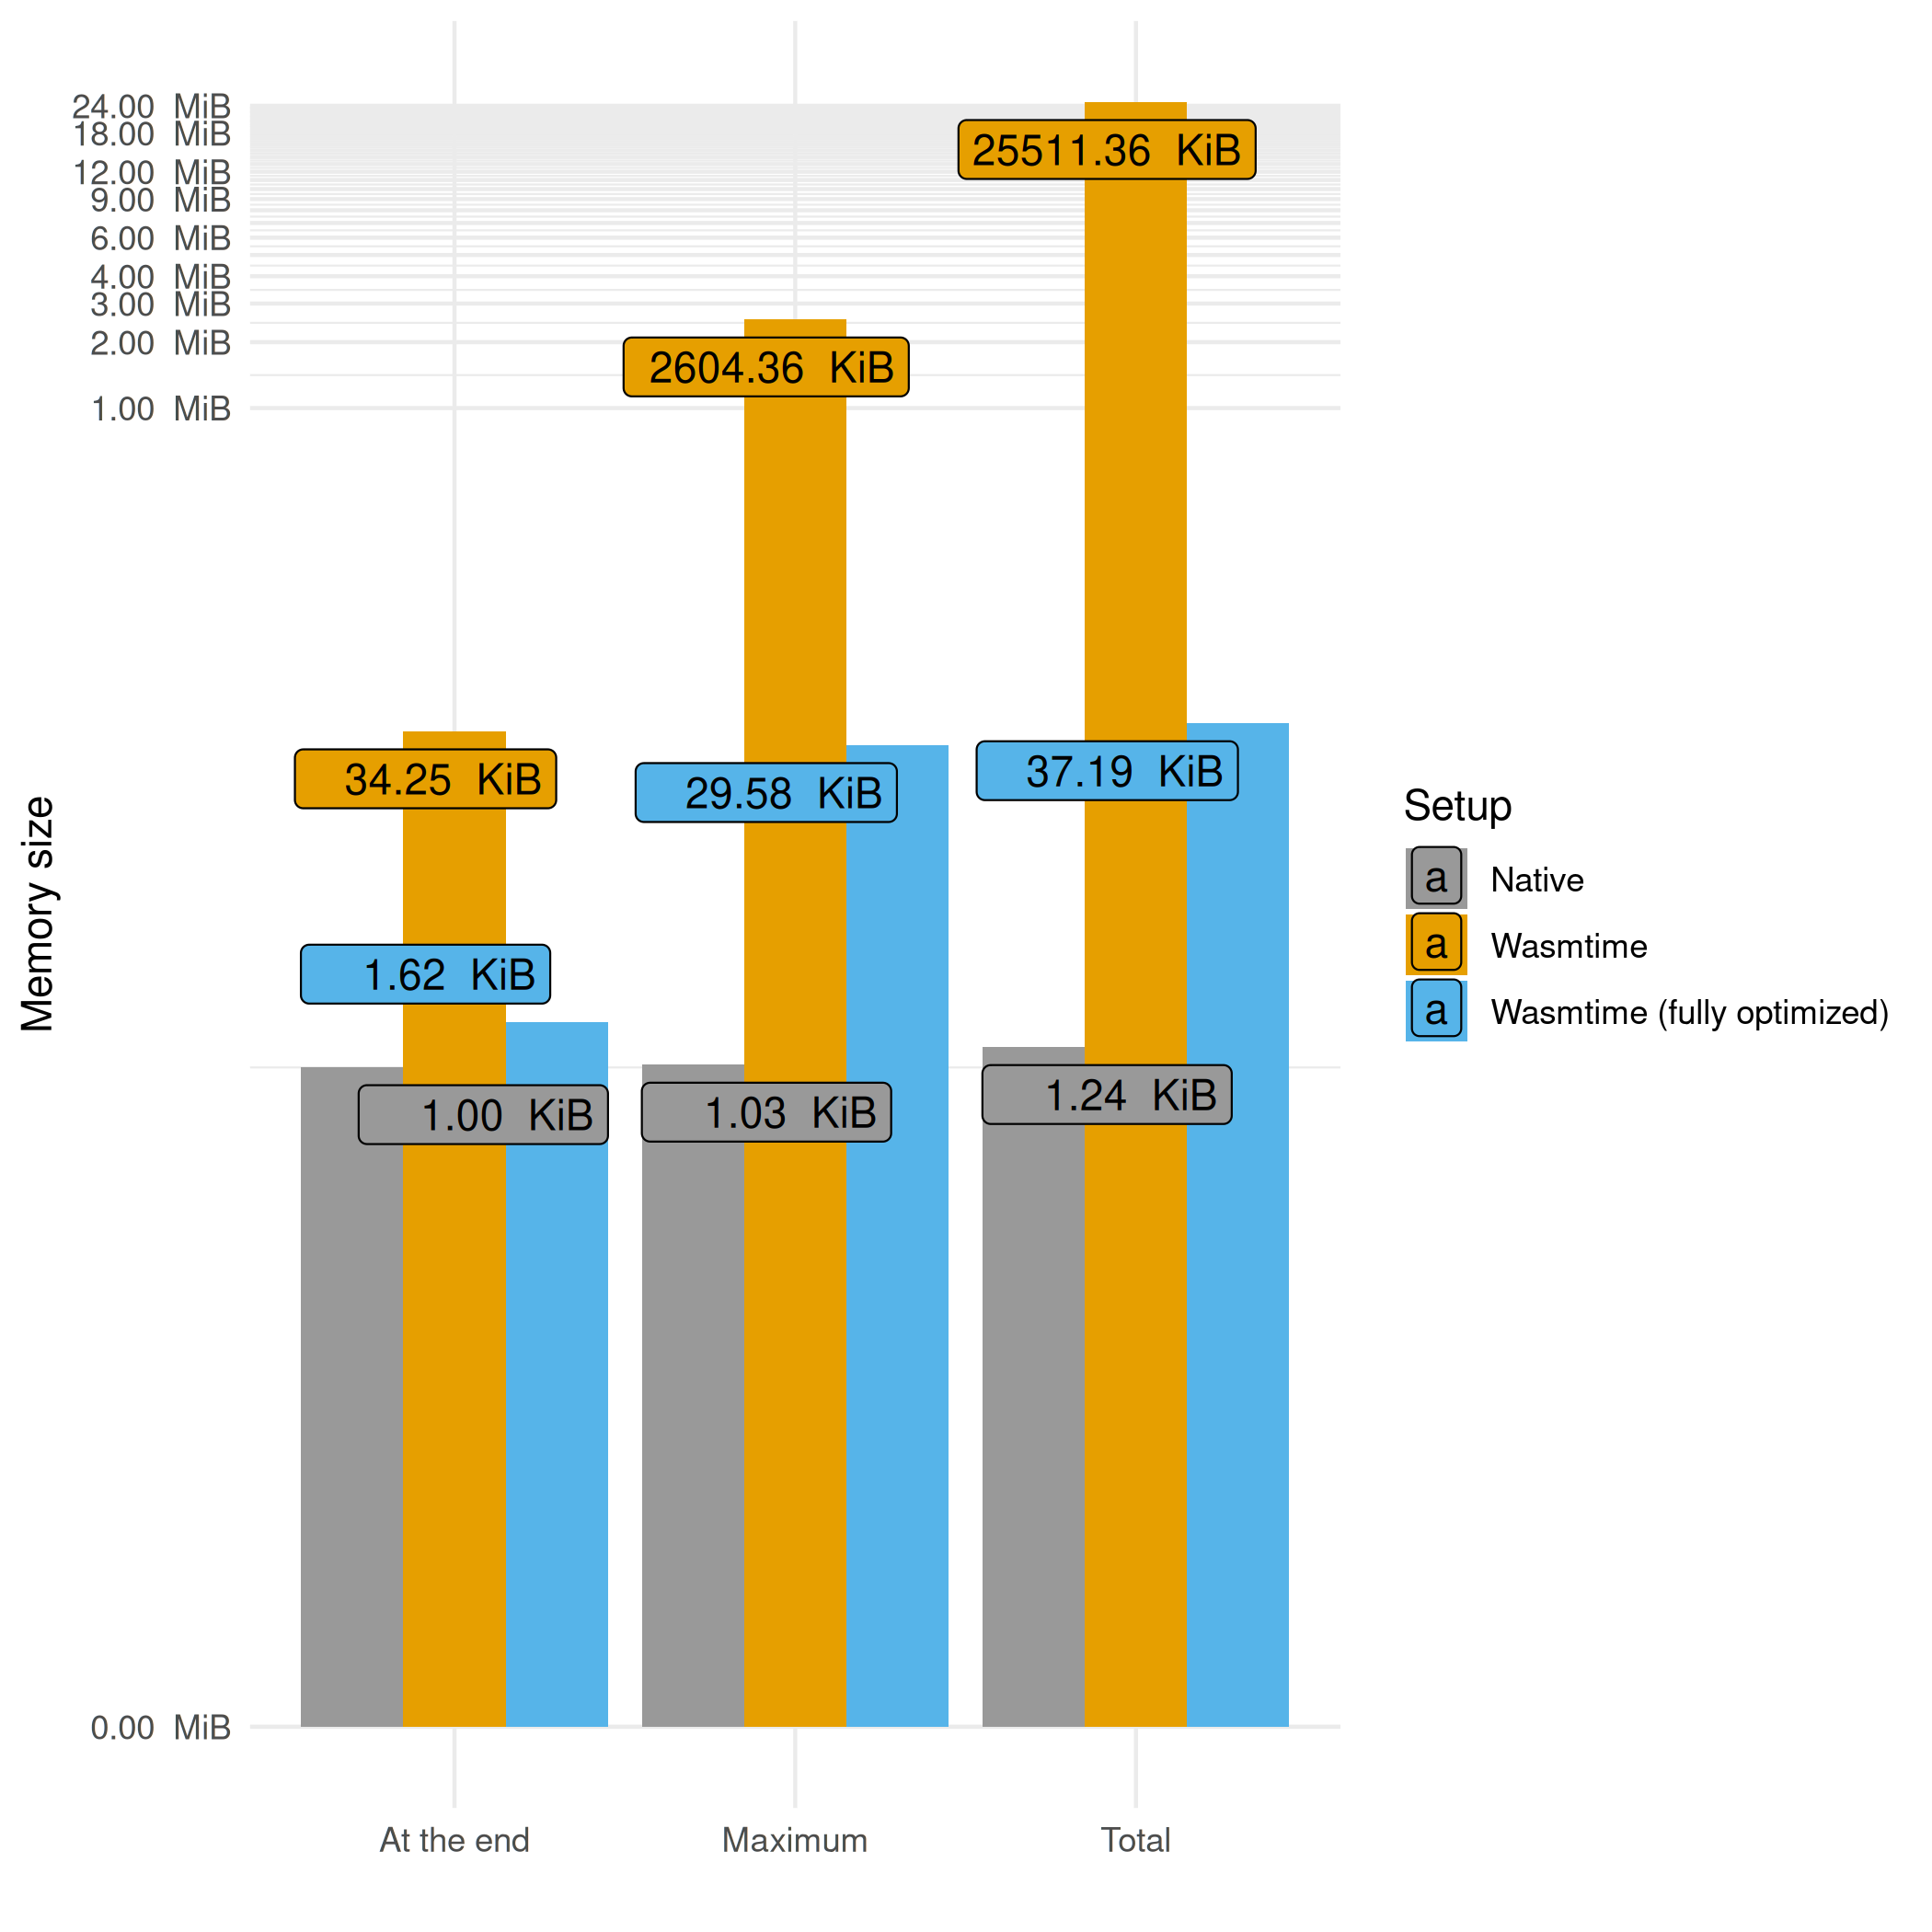
\includegraphics[width=\linewidth]{figures/sensor_memory}
  \caption{Reading from the sensor.}
\end{subfigure}%
\begin{subfigure}{.5\textwidth}
  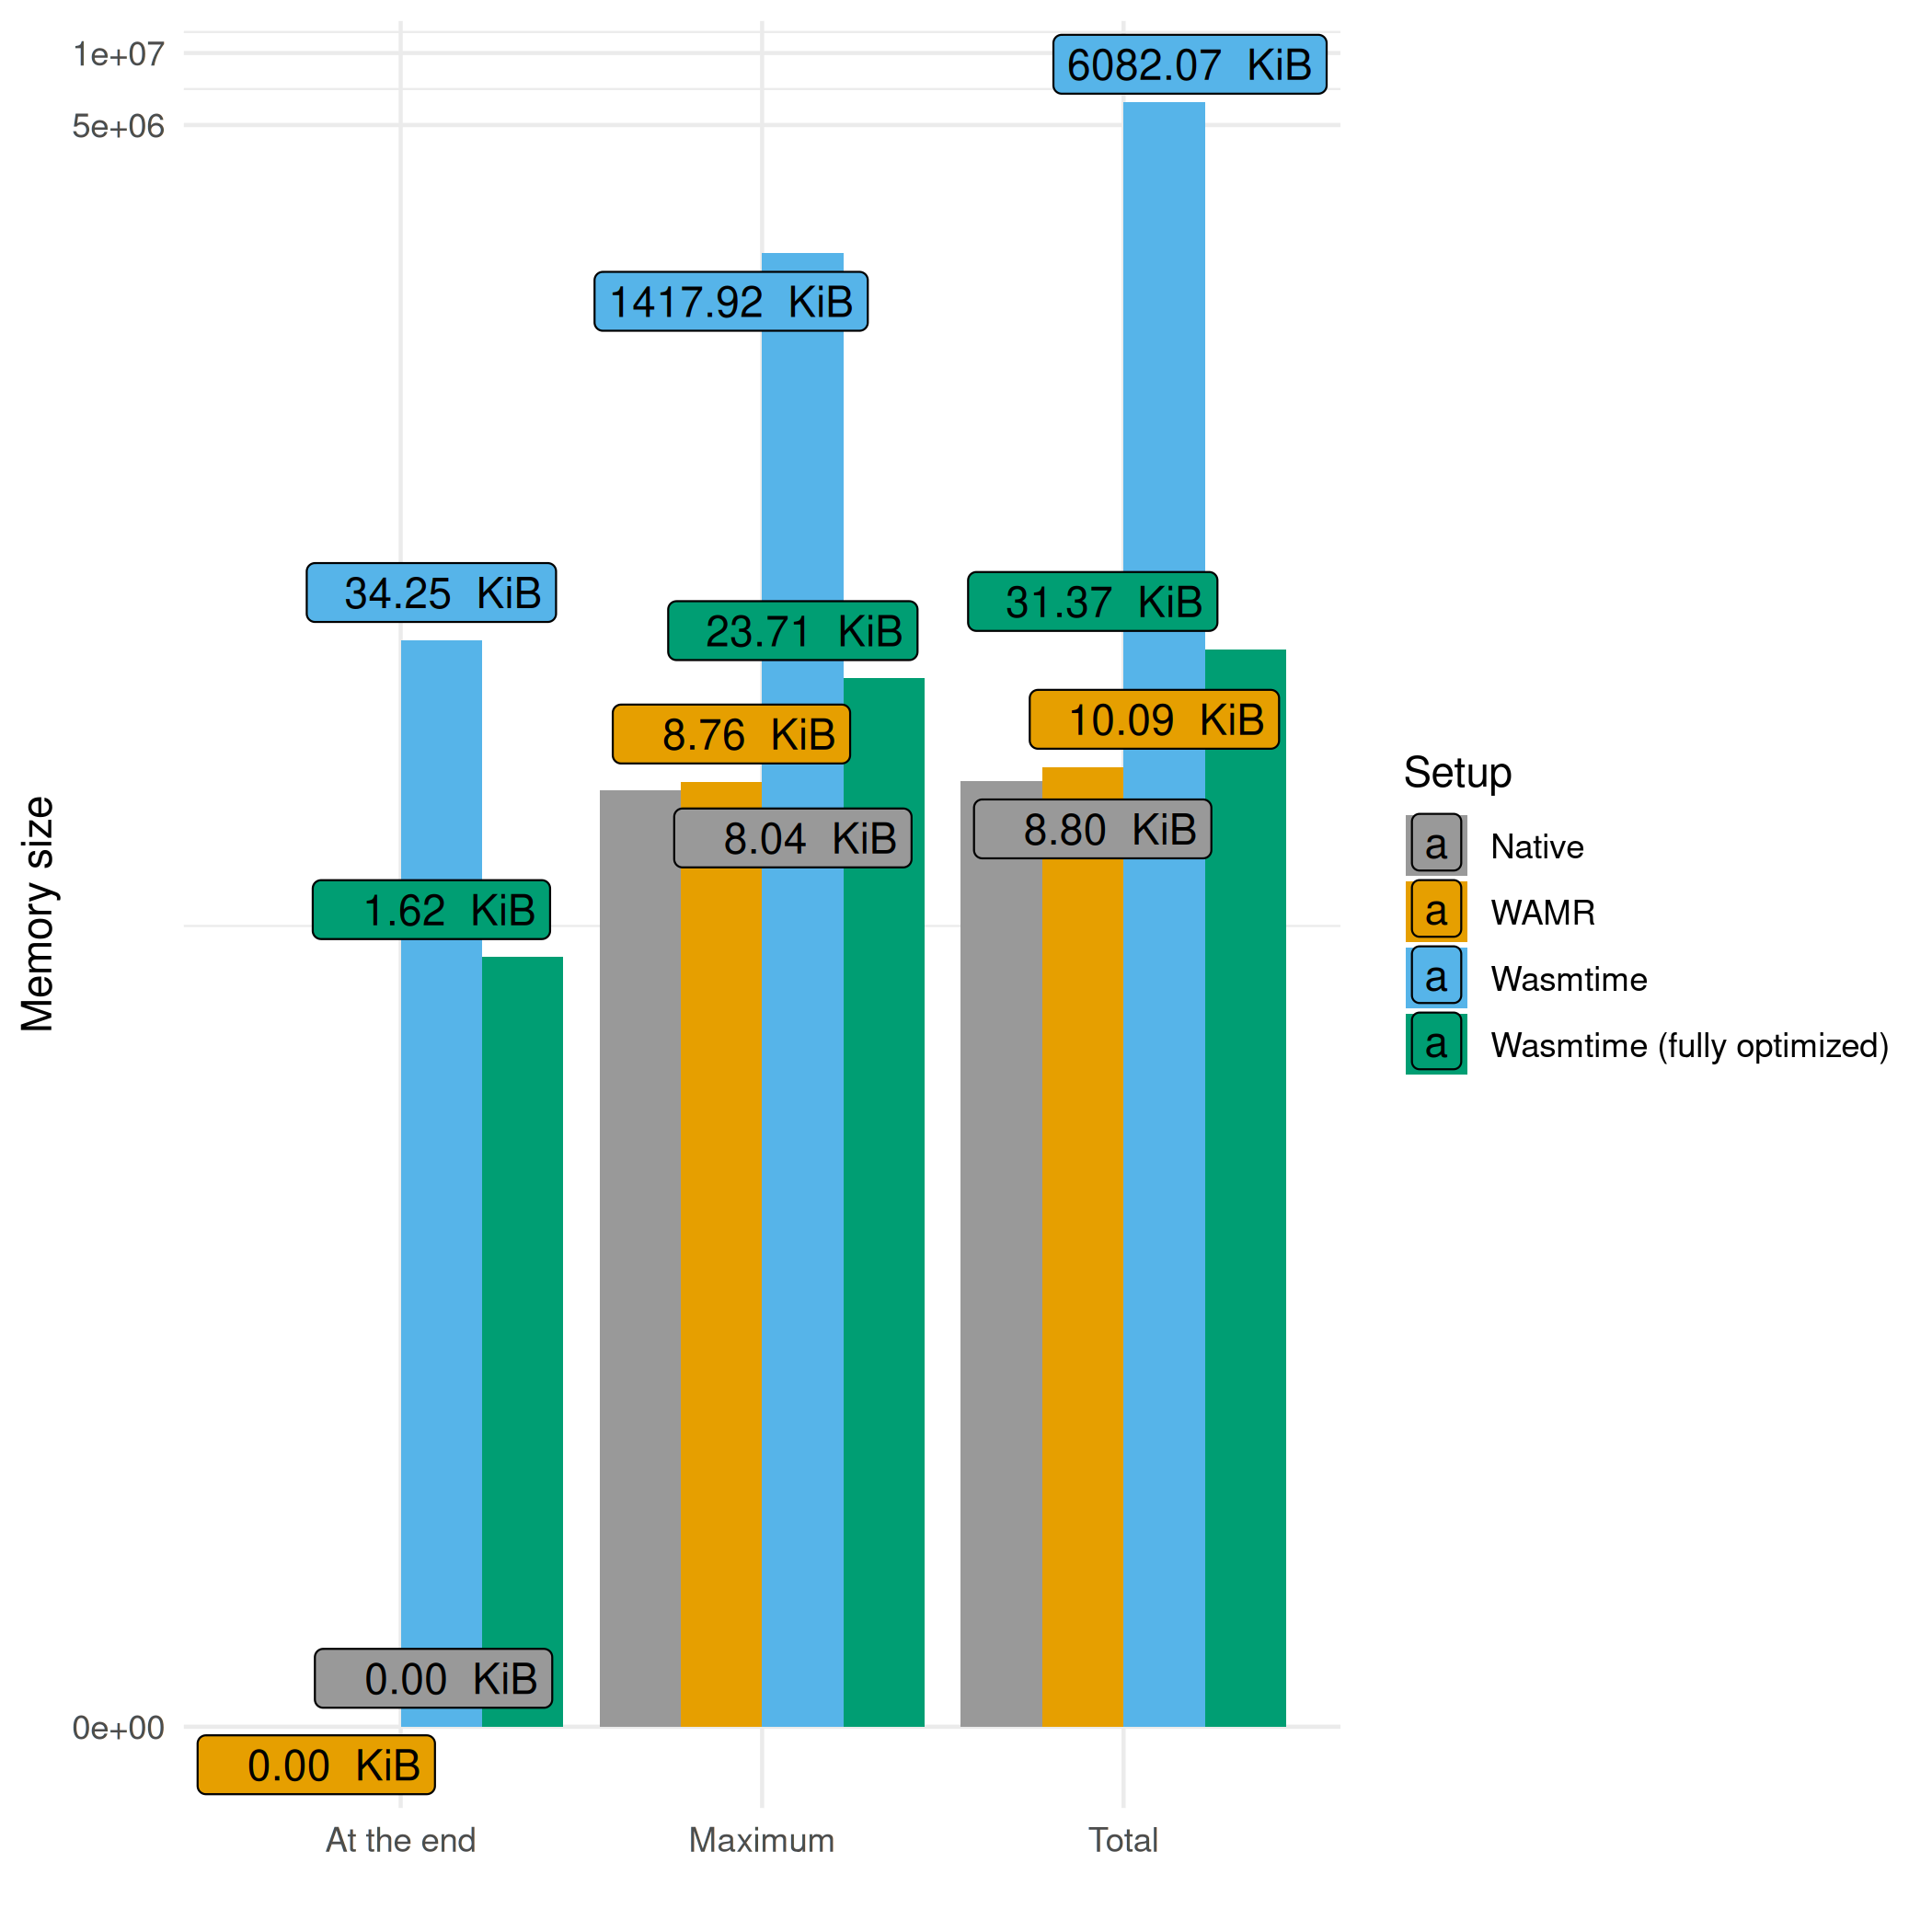
\includegraphics[width=\linewidth]{figures/display_memory}
  \caption{Writing to the display.}
\end{subfigure}%
\caption{Used memory size when...}
  \label{fig:mem}
\end{figure}

% \begin{table}[h]
% 	\centering
% 	\captionsetup{justification=centering}
% 	% \label{tab:criteria}
% 	\begin{tabular}{l c c c}
% 		\toprule
%                   & Total & Maximum & At the end \\ \midrule
%       Native    & 8.8 KiB & 8.4 KiB & 0 B \\
%       Wasmtime  &  5.94 MiB & 1.39 MiB & 34.25 KiB \\
%       Wasmtime (fully optimized) & 31.17 KiB & 23.71 KiB & 1.62 KiB \\
%       WAMR  &  10.9 KiB & 8.76 KiB & 0 B \\
% 		\bottomrule
% 	\end{tabular}
%     \caption{Used memory for writing to the display}
% \end{table}

% \begin{table}[h]
% 	\centering
% 	\captionsetup{justification=centering}
% 	% \label{tab:criteria}
% 	\begin{tabular}{l c c c}
% 		\toprule
%                   & Total & Maximum & At the end \\ \midrule
%       Native    & 1.24 KiB & 1.03 KiB & 1 KiB \\
%       Wasmtime  & 24.67 MiB & 2.66 MiB & 34.25 KiB \\
%       Wasmtime (fully optimized) &  37.19 KiB & 29.58 KiB & 1.62 KiB \\
% 		\bottomrule
% 	\end{tabular}
%     \caption{Used memory for reading from the sensor}
% \end{table}

When considering the memory usage, Figure~\ref{fig:mem}, three phenomena are striking. First, the performed optimizations to make the Wasmtime implementation run faster also greatly benefit the memory usage. Second, WAMR has near-native memory usage, while Wasmtime uses nearly four times more memory when compared to the native version. Third and last, the memory usage of the fully optimized version of Wasmtime is fairly similar between writing to the display and reading from the sensor. This showcases a baseline amount of memory required to run the component model.

To conclude, both solutions for Wasmtime greatly benefitted from precompiling the Wasm binary. Furthermore, precompilation makes Wasmtime on par with WAMR and native time-wise, but Wasmtime still requires a substantial larger amount of memory to succesfully run.

\begin{sidewaysfigure}
  \begin{subfigure}{\linewidth}
    \centering
    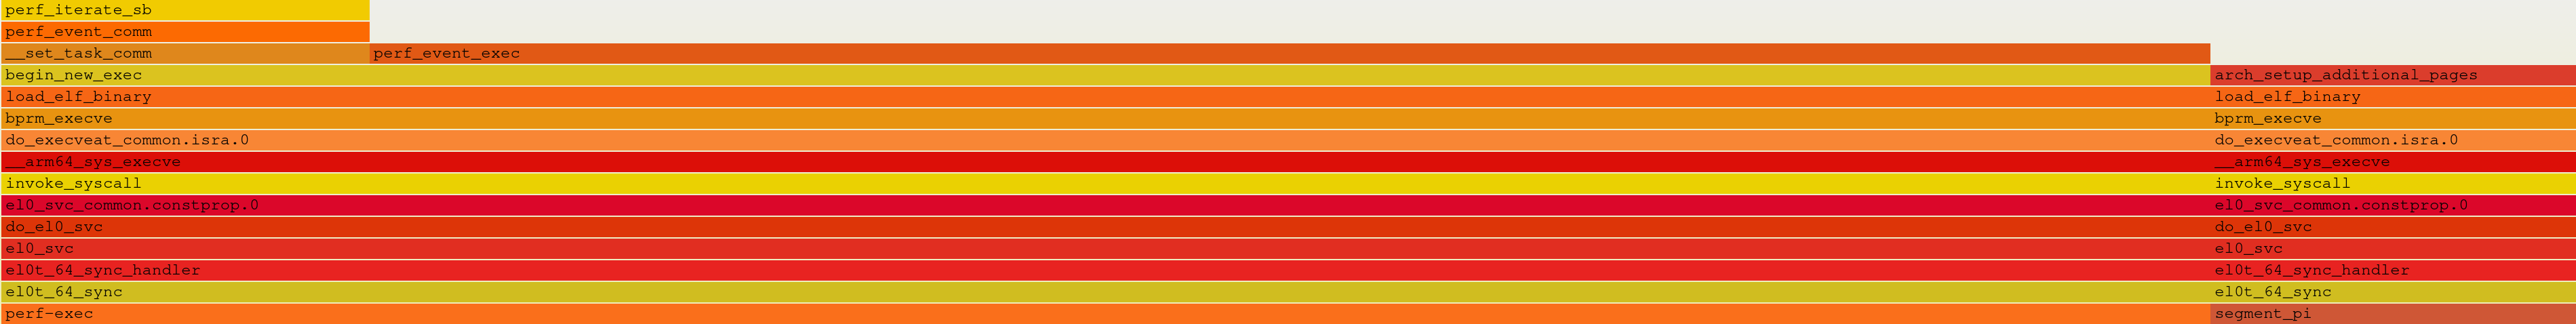
\includegraphics[width=\textwidth]{figures/native_led_flamegraph}
    \caption{Native}
    \label{fig:flamegraph:led:native}
  \end{subfigure}
  \begin{subfigure}{\linewidth}
    \centering
    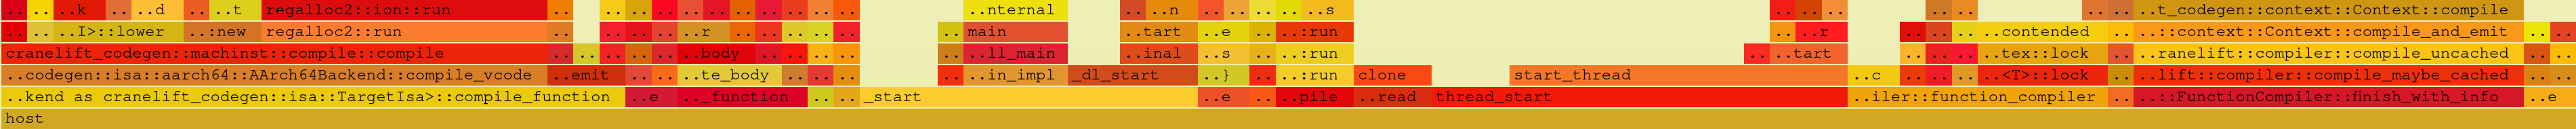
\includegraphics[width=\textwidth]{figures/wasmtime_flamegraph}
    \caption{Inside Wasmtime}
    \label{fig:flamegraph:wasmtime}
  \end{subfigure}
  \begin{subfigure}{\linewidth}
    \centering
    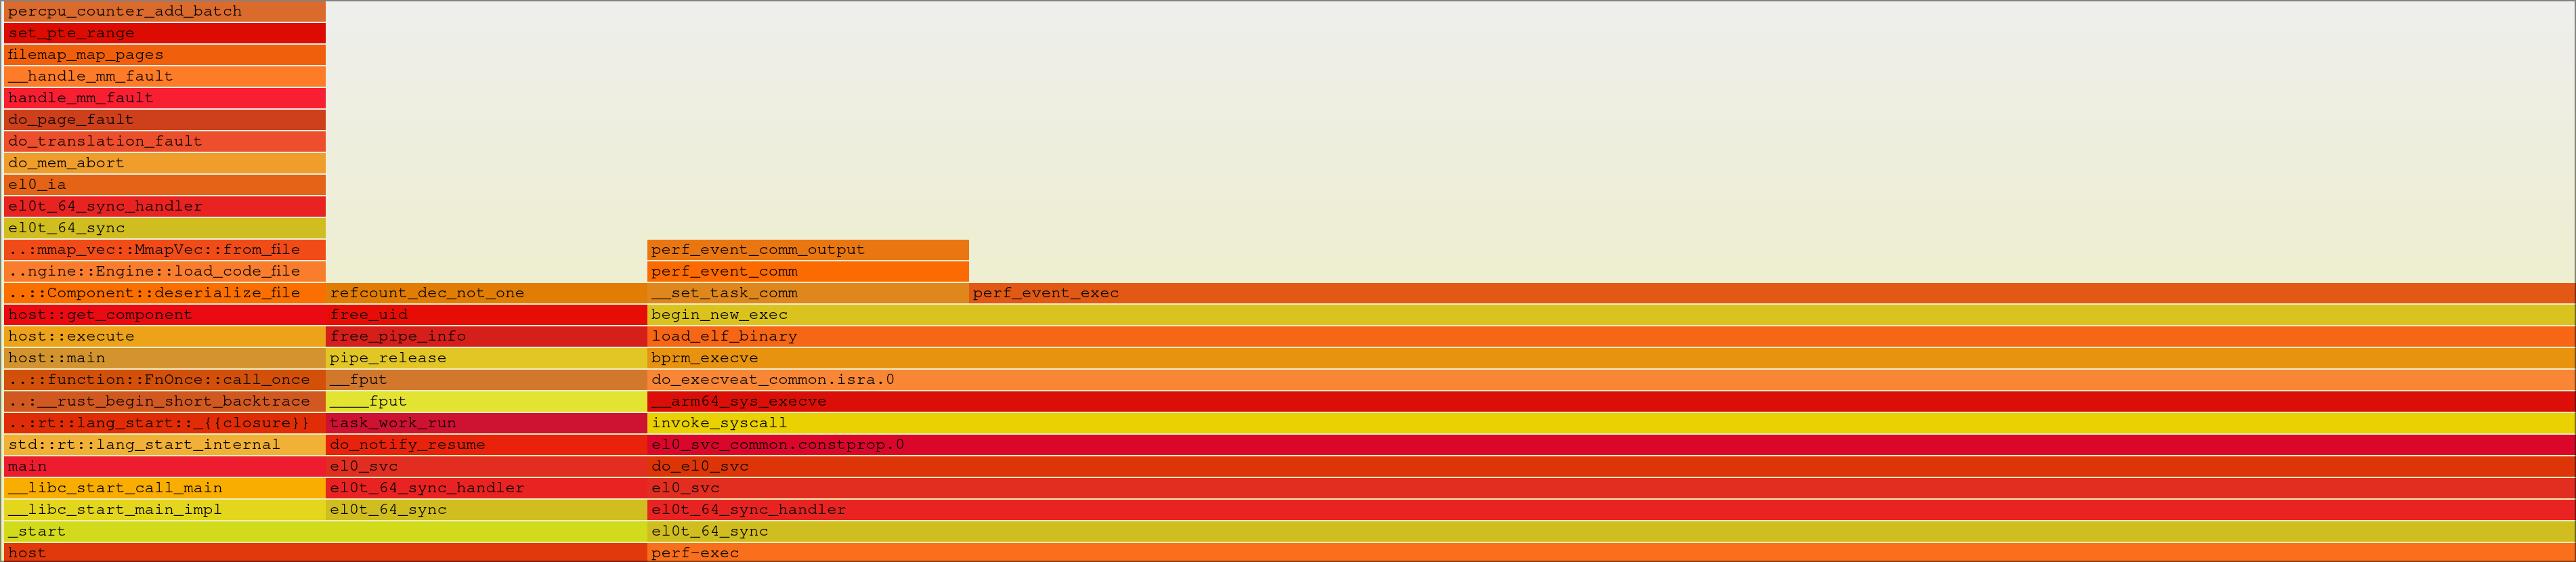
\includegraphics[width=\textwidth]{figures/optim_led_flamegraph}
    \caption{Inside Wasmtime (precompiled binary \& without command world)}
    \label{fig:flamegraph:led:compiled}
  \end{subfigure}
  \begin{subfigure}{\linewidth}
    \centering
    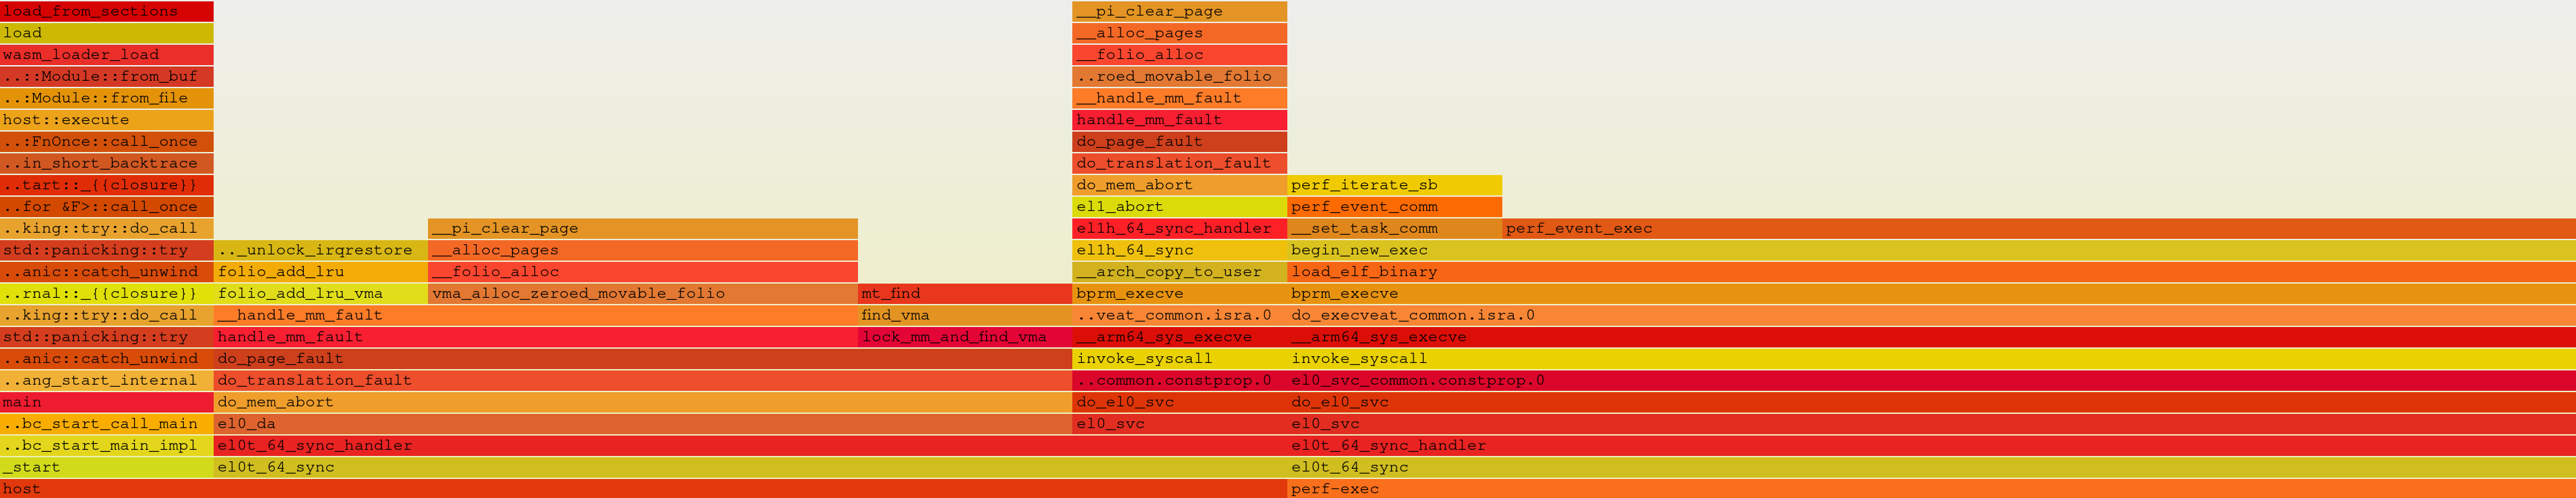
\includegraphics[width=\textwidth]{figures/wamr_led_flamegraph}
    \caption{Inside WAMR}
    \label{fig:flamegraph:led:wamr}
  \end{subfigure}
  \caption{Flamegraphs of writing to the display}
\end{sidewaysfigure}

\begin{sidewaysfigure}
  \centering
  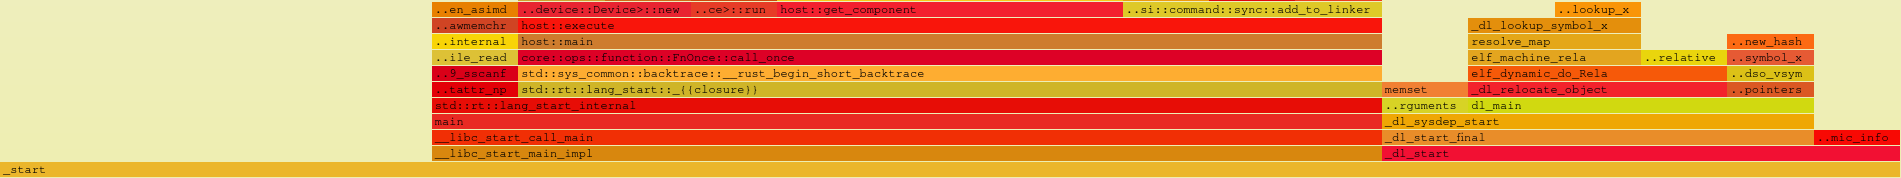
\includegraphics[width=\textwidth,keepaspectratio]{figures/compiled_sensor_flamegraph}
  \caption{Flamegraph of reading the sensor inside Wasmtime with a precompiled component.}
  \label{fig:flamegraph:sensor}
\end{sidewaysfigure}



% Moet zeker goed verwoord zijn
\chapter*{Conclusie}
\chaptermark{Conclusie}
\addcontentsline{toc}{chapter}{Conclusie}  

[Terugblikken naar de introductie en wat ik allemaal bijgeleerd heb.]

Vertellen over SPI.
[Het nog verder advancen van de proposal enbespreken van dingen waar ik niet klaar mee geraakt ben.]

\renewcommand\bibname{References}
\bibliography{references}


\pagestyle{numberless} 
\pagestyle{empty}
\begin{appendices}
\section*{Bijlage A}
\addcontentsline{toc}{section}{Bijlage A}  

Toelichting bijlage.



\newpage
\section*{Bijlage B}
\addcontentsline{toc}{section}{Bijlage B}  

Toelichting bijlage.

\end{appendices}


\end{document}
